\chapter{Experimentation and comparison}
\label{chap:experiments}

Chapter~\ref{chap:approach} proposed a genetic-programming hyper-heuristic
(GPHH) baseline and a family of candidate modifications to it. This chapter
reports how those candidates were actually evaluated, and, just as
importantly, how the space of candidates was narrowed before any of them
was evaluated at full scale. The experimental programme underlying this
chapter was carried out in two clearly separated stages. An
\emph{exploratory} stage (Section~\ref{sec:parameter-sensitivity}) screened
a wide range of algorithmic ideas cheaply, using small populations, few
generations and few benchmark instances, with the explicit purpose of
generating and discarding hypotheses rather than producing publishable
numbers. A \emph{comprehensive} stage (Section~\ref{sec:operator-evaluation})
then took the small number of ideas that survived screening and evaluated
them at the scale, statistical power and instance coverage required to
support a scientific claim. Rather than evaluating every idea exhaustively,
preliminary experiments were first used to identify promising research
directions, and only those directions were carried forward into the
expensive, fully powered study. \changed{Two terms are used with a fixed
meaning throughout this chapter: a \emph{condition} is one algorithm
configuration under comparison (the baseline, or the baseline with one
proposed modification applied), and a \emph{cell} is one combination of
schedule generation scheme and GP decision strategy; every condition is
evaluated in every cell, on both benchmark datasets, with 30 random seeds
each.}

\section{Software implementation}
\label{sec:software-implementation}

All experiments were run against a single, shared code base
(\texttt{GP\_MRCPSP\_CEC2024/yuantian}) built on top of Tian, Mei and
Zhang's own reference implementation~\cite{Tian2024GPHH}, using
DEAP~\cite{derainville2012deap} for the underlying evolutionary loop
(population handling, crossover, mutation, and the tree representation
itself) and the \texttt{discrete-optimization} library for canonical
schedule decoding and feasibility checking. Every configuration compared in
this chapter, baseline and every proposed modification alike, therefore
shares the same GP engine, the same multi-tree individual representation
(Section~\ref{subsec:individual-representation}), the same instance parser,
and the same fitness computation; configurations differ only in the
specific, additive change under test (selection operator, elite refinement
step, or terminal set), so that a difference in outcome can be attributed
to that change rather than to incidental implementation drift between
otherwise-unrelated codebases.

The exploratory and comprehensive stages are implemented as two separate,
purpose-built harnesses within this shared code base. \changed{For clarity
of attribution: the \texttt{yuantian/} directory vendors \changedC{Tian,
Mei and Zhang's reference implementation~\cite{Tian2024GPHH}}, and everything evaluated in this chapter beyond
the plain baseline, the \texttt{exploratory/} and \texttt{experiments/}
modules and every extension condition, is this thesis's own addition
inside that directory, kept there so that the extensions and the reference
implementation share one code and import structure.}
\changed{Section~\ref{sec:parameter-sensitivity}'s pilot experiments are driven by
\texttt{yuantian/exploratory/} (one module per screened mechanism): the
DMGE-family comparison via
\texttt{yuantian/experiments/exploratory\_sweep\_experiment.py}, and the
staged lexicase/local-search evaluation via
\texttt{lexicase\_local\_search\_experiment.py} and
\texttt{full\_mmlib\_experiment.py}.}
Section~\ref{sec:operator-evaluation}'s comprehensive evaluation is driven
by a single \emph{matrix} experiment,
\texttt{yuantian/experiments/matrix\_runner.py}, parameterised by condition
(baseline, lexicase, local search, hybrid, NR terminals, and NR terminals'
own matched control), GP decision strategy (activity-first, mode-first,
simultaneous), schedule generation scheme (serial, parallel), benchmark
dataset, and random seed; \texttt{matrix\_config.py} is the single source
of truth for this grid and for the fixed parameter values reported in
Table~\ref{tab:experimental-parameters}. Because the full grid at the
paper's own population and generation budget is computationally heavy, runs
were distributed as PBS array jobs on the MetaCentrum computing grid
(Section~\ref{subsec:hw-sw}), and results were aggregated and tested for
significance offline with \texttt{yuantian/experiments/analyze\_matrix.py}
and \texttt{final\_comparison\_report.py}, which implement the statistical
methodology of Section~\ref{subsec:statistical-methodology} uniformly
across every condition and dataset.

\section{Experimental setup}
\label{sec:experimental-setup}

This section fixes the experimental protocol used throughout the rest of
the chapter: the hardware and software environment, the benchmark
instances and how they were sampled, the algorithm's parameters, the number
of independent runs, the evaluation metric, and the statistical procedure
used to decide whether an observed difference is meaningful. The same
protocol is used, without modification, for the exploratory and the
comprehensive stage; only the scale (population size, generation count,
instance count, and seed count) differs between them, as detailed in each
stage's own section.

\subsection{Hardware and software environment}
\label{subsec:hw-sw}

\changed{All runs were executed on the MetaCentrum national computing
grid. Table~\ref{tab:hw-sw-config} summarises the software environment,
the per-job resource allocation, and how jobs were scheduled.}

\begin{table}[htbp]
  \centering
  \small
  \caption[Hardware and software configuration]{\changed{Hardware and
  software configuration used for the runs reported in this chapter.
  Individual jobs were placed by the PBS scheduler on whichever grid nodes
  were available, so the exact hardware varies from run to run; the
  submission environment and per-job resource allocation below were
  constant.}}
  \label{tab:hw-sw-config}
  \begin{tabular}{@{}p{0.27\textwidth}p{0.65\textwidth}@{}}
    \toprule
    \textbf{Component} & \textbf{Configuration} \\
    \midrule
    Compute platform & MetaCentrum national computing grid (OpenPBS scheduler, version 23.06.06) \\
    \changed{Submission host} & \changed{\texttt{tarkil.grid.cesnet.cz}; compute nodes assigned per job by the scheduler (heterogeneous hardware)} \\
    Per-job allocation & 1 node, 8 CPU cores, 8\,GB RAM, 8\,GB local scratch \\
    Parallelism & population evaluation parallelised across 8 cores per run (\texttt{--multiprocess}) \\
    \changed{Operating system} & \changed{Debian GNU/Linux 12 (``bookworm'') on the submission host; node OS varies with the assigned machine} \\
    Python & 3.11.2, loaded via module \texttt{python/\allowbreak3.11.11-\allowbreak gcc-\allowbreak 10.2.1-\allowbreak 555dlyc} \\
    Core libraries & DEAP~\cite{derainville2012deap}, \texttt{discrete-optimization}, NumPy 1.24.2, SciPy \\
    Job scheduling & one PBS array element per (condition, strategy, SGS, dataset, seed) combination \\
    \bottomrule
  \end{tabular}
\end{table}

\subsection{Benchmark datasets and instance sampling}
\label{subsec:instance-sampling}

Both the exploratory and the comprehensive stage draw instances from
MMLIB50 and MMLIB100 (Section~\ref{subsec:mmlib}). \changed{Each MMLIB
dataset consists of 108 instance classes of five instances each, where a
class is one combination of the generator's OS/RF/RS target levels
(Section~\ref{subsec:indicators}). Following Tian et al.'s 60/20/20
convention, the five instances of every class are split into three
training instances, one validation instance and one test instance, so a
run trained on $n_{\text{classes}}$ classes sees $3\,n_{\text{classes}}$
training instances and is tested on $n_{\text{classes}}$ held-out ones.
\changed{The training, validation and test instances of a class therefore
always share the same OS/RF/RS setting: generalisation is measured to
\emph{unseen instances with the same characteristics}, not to unseen
characteristics.}
All planned runs of the comprehensive stage were completed, but on a
stratified subset of $n_{\text{classes}}=10$ classes, evenly spaced across
each dataset's class-index range (class indices $1, 11, 21, \dots, 91$)
and identical for every condition and
every seed, so that the subsampling cannot bias the comparison between
conditions. Because MMLIB numbers its classes systematically along the
generator's OS/RF/RS parameter grid, an even stride over the class indices
samples across the whole range of instance characteristics rather than
clustering in one region (the selected classes cover
$\mathrm{OS} \in \{0.25, 0.5, 0.75\}$, $\mathrm{RF} \in \{0.5, 1.0\}$
and RS from tight to effectively unconstrained,
cf.\ Table~\ref{tab:per-class-breakdown}); \changedC{it is, however, a
deterministic stride and does not guarantee that every OS/RF/RS
combination receives a class, so some parameter combinations are
unrepresented;} evaluating on all 108 classes at the paper's population and
generation budget would have required an estimated several hundred days of
computation\changedC{, which could not have been completed within the time
frame of this thesis}.}
Table~\ref{tab:experimental-parameters}
records this together with the remaining fixed settings.

\subsection{Algorithm parameters}
\label{subsec:algorithm-parameters}

\changed{Table~\ref{tab:experimental-parameters} lists the fixed parameter
values used throughout the comprehensive stage; except for the reduced
class count $n_{\text{classes}}$, they match the configuration of Tian et
al.~\cite{Tian2024GPHH}.}

\begin{table}[htbp]
  \centering
  \small
  \caption[Experimental parameters]{Fixed parameter values used throughout
  the comprehensive evaluation stage (Section~\ref{sec:operator-evaluation}).
  These match Tian et al.'s~\cite{Tian2024GPHH} own reported configuration
  except for $n_{\text{classes}}$, which is reduced from the paper's full
  108-class split for computational tractability
  (Section~\ref{subsec:instance-sampling}); the exploratory stage
  (Section~\ref{sec:parameter-sensitivity}) instead uses a substantially
  smaller population, generation count and instance count, since its purpose
  is cheap screening rather than a publishable estimate.}
  \label{tab:experimental-parameters}
  \begin{tabular}{@{}p{0.55\textwidth}p{0.35\textwidth}@{}}
    \toprule
    \textbf{Parameter} & \textbf{Value} \\
    \midrule
    Population size & 1\,000 \\
    Generations & 50 \\
    Elite individuals carried forward & 10 \\
    Tournament size (baseline selection) & 7 \\
    Crossover rate / mutation rate & 0.80 / 0.15 \\
    Maximum tree depth & 8 \\
    Initial tree depth range (ramped half-and-half) & 2--6 \\
    Local search elite fraction / iterations & 8\% pop.\ / 10 iterations \\
    Stratified classes per dataset ($n_{\text{classes}}$) & 10 (of 108) \\
    Train / validation / test cases per class & 3 / 1 / 1 \\
    Independent seeds per configuration & 30 \\
    Seed range (comprehensive stage) & 12\,000--12\,029 \\
    \bottomrule
  \end{tabular}
\end{table}

\subsection{Independent runs and evaluation metric}
\label{subsec:runs-and-metric}

Every reported configuration (a condition, GP decision strategy and
schedule generation scheme combination) is repeated for 30 independent
random seeds in the comprehensive stage, matching the seed count used by
Tian et al.\ for Tables V and VI of the source paper and giving each
comparison a paired sample of 30 observations. The evaluation metric
throughout is the Average Relative Deviation (ARD\%) from the CPM lower
bound, defined in Section~\ref{sec:eval-metrics}; both the training-set ARD\%
(the quantity the GP search directly minimises) and the held-out test-set
ARD\% (the quantity that actually matters for generalisation) are reported
side by side wherever the two diverge in an interesting way, since a method
that only improves training fitness is not, on its own, evidence of a
better learned heuristic.

\subsection{Statistical methodology}
\label{subsec:statistical-methodology}

\changed{Table~\ref{tab:statistical-methodology} summarises the statistical
procedures applied uniformly to every comparison in this chapter; the
paragraphs below define them in detail.}

\begin{table}[htbp]
  \centering
  \small
  \caption[Statistical methodology]{Statistical procedures applied uniformly
  to every comparison in this chapter.}
  \label{tab:statistical-methodology}
  \begin{tabular}{@{}p{0.32\textwidth}p{0.58\textwidth}@{}}
    \toprule
    \textbf{Aspect} & \textbf{Procedure} \\
    \midrule
    Paired comparison (condition vs.\ baseline) & Wilcoxon signed-rank test, two-sided, $\alpha = 0.05$ \\
    Pairing unit & random seed (same stratified instance split across conditions) \\
    Effect size & matched rank-biserial correlation $r \in [-1, 1]$ \\
    Feasibility handling & per-instance feasible-only mean; a seed is dropped only if \emph{zero} instances were feasible under it (Section~\ref{sec:eval-metrics}) \\
    Multi-condition ranking & Friedman test across (SGS, decision strategy) cells as blocks, with average rank per condition, visualised as a critical-difference diagram \\
    Multiple comparisons & \emph{not} corrected for family-wise error across cells (Section~\ref{subsec:threats-stat}) \\
    \bottomrule
  \end{tabular}
\end{table}

Two comparisons recur throughout this chapter and are always reported
together: a \emph{pairwise} test (a candidate condition against its
baseline, one SGS/strategy cell at a time) and, where three or more
conditions are compared jointly (Section~\ref{subsec:final-comparison}), a
\emph{joint ranking} across cells. For the pairwise case, each cell's 30
seeds give 30 paired (baseline, condition) observations; a Wilcoxon
signed-rank test on these pairs is reported together with the matched
rank-biserial effect size $r$, which is signed so that $r>0$ means the
candidate condition achieved lower (better) ARD\% than baseline and $r<0$
means the opposite. For the joint-ranking case, each of the six (SGS,
strategy) cells contributes one observation per condition (that cell's mean
ARD\% under that condition), conditions are ranked 1 (best) to $k$ (worst)
within each cell, and a Friedman test on these ranks (blocks = cells)
checks whether the average ranks differ by more than chance.

\textbf{Boxplots.} Where referenced below, a boxplot shows the distribution
of a metric (typically test-set ARD\%) across the 30 seeds of a given
configuration: the box spans the interquartile range, the line inside it
is the median, whiskers extend to the most extreme non-outlier
observations, and individual points beyond the whiskers are plotted as
outliers. Boxplots are the primary way this chapter communicates
\emph{spread}, not just the mean reported in text: two configurations with
identical means but very different spreads represent a materially
different practical proposition (a consistently mediocre method versus an
unreliable but occasionally excellent one), and the mean/std pairs in the
descriptive-statistics tables alone can obscure that distinction.

\textbf{Critical-difference (CD) diagrams.} Where referenced below, a
critical-difference diagram plots each condition's average rank (as defined
above) on a shared axis and draws a bold horizontal bar connecting any
group of conditions whose average ranks are \emph{not} statistically
distinguishable at the chosen significance level, following the
convention popularised for classifier comparison by
Dem\v{s}ar~\cite{demsar2006}. A CD diagram
is reported only where the corresponding Friedman test is itself
significant; where it is not, the ranking is reported as a plain table
instead, since drawing a CD diagram over ranks that a Friedman test could
not distinguish from chance would visually overstate the evidence for a
difference between individual conditions' averaged ranks. \changed{Note
that the joint ranking has only the six (SGS, strategy) cells available as
blocks, which limits the resolution of the Friedman test and makes the
critical difference wide; this limitation is discussed together with the
other statistical caveats in the conclusion.}

\subsection{Reproducibility}
\label{subsec:reproducibility}

Every result file records enough information to be regenerated
independently: which of \texttt{matrix\_config.py}'s (condition, strategy,
SGS, dataset) cells it belongs to, the exact random seed, and per-instance
feasibility and fitness records for both the training and the held-out test
set. PBS array jobs read one row per array index from a checked-in
manifest CSV (\texttt{pbs\_jobs/*.manifest.csv}), so any individual cell can
be re-submitted in isolation; a completed result already present at the
persistent output location is not recomputed. \changed{One practical note
for re-running: the experiment scripts should be executed with
\texttt{python -O}, since the parallel simulator contains
\texttt{\_\_debug\_\_}-guarded diagnostic printing that otherwise floods
the logs.} The analysis scripts
(Section~\ref{sec:software-implementation}) are themselves committed to the
repository, so the numbers reported in
Sections~\ref{sec:operator-evaluation} and~\ref{sec:benchmark-comparison}
can be regenerated from the raw per-seed result files without re-running any
GP search. \changed{The exact version of the codebase used to produce all
results reported in this chapter, including the raw per-seed result files
themselves, is archived under the git tag \texttt{thesis-results} (commit
\texttt{a817f90}) and is publicly available at
\changedC{\url{https://github.com/sabinasagova/master-thesis/releases/tag/thesis-results}}.}

\section{Operator and local search evaluation}
\label{sec:operator-evaluation}

The pilot phase of Section~\ref{sec:parameter-sensitivity} narrowed a wide
field of candidate modifications down to three that were judged worth a
full, fully powered evaluation: epsilon-lexicase selection
(Section~\ref{subsec:lexicase-eval}), a critical-path-guided \changed{Baldwinian}
local search applied to elite individuals
(Section~\ref{subsec:localsearch-eval}), and a set of terminals exposing
non-renewable resource state to the GP
(Section~\ref{subsec:nr-eval}). Each is now compared against its matched
baseline at the full protocol of Section~\ref{sec:experimental-setup}: 30
seeds, population 1\,000, 50 generations, \changed{all three GP decision
strategies (activity-first, mode-first, simultaneous\changedC{, defined in
Section~\ref{subsec:individual-representation}}) and both schedule
generation schemes (serial and parallel\changedC{,
Section~\ref{subsec:sgs}}).}

This evaluation is run at full scale on \emph{both} benchmark sets, which
play complementary roles. \textbf{MMLIB50 is this thesis's primary evidence
base}: \changed{the full experiment grid, 6 conditions (baseline, lexicase,
local search, hybrid, NR terminals, and NR terminals' matched control
\texttt{baseline\_nr}) $\times$ 3 decision strategies $\times$ 2 schedule
generation schemes $\times$ 30 seeds $= 1\,080$ runs, is complete} and is
what each subsection's main
discussion is built on. \textbf{MMLIB100 is this thesis's scalability
validation at the same full scale}: doubling the number of activities per
instance roughly doubles the size of the precedence graph and the
combinatorial mode-assignment space the GP rule has to generalise over, so
\changed{MMLIB100 is where this thesis checks whether the MMLIB50 findings
are properties of the underlying mechanisms or artefacts of MMLIB50's
specific instance scale.} MMLIB100's grid is likewise complete (1\,080 of 1\,080
runs). Every subsection below therefore reports MMLIB100's real numbers
directly alongside MMLIB50's, under its own ``Scalability validation''
heading, with generated boxplots and, where the underlying Friedman test is
significant, critical-difference diagrams for both benchmark sets. In every
comparison table, a direction marker next to a condition's mean summarises
its change against the matched baseline in the same row:
\ArrBetter{} marks lower (better) ARD\%, \ArrWorse{} marks higher (worse)
ARD\%, and \ArrSame{} marks a mean equal to the baseline's at the reported
precision.

\subsection{Comprehensive evaluation of lexicase selection}
\label{subsec:lexicase-eval}

Epsilon-lexicase selection (defined in full in
Section~\ref{subsec:lexicase-definition}) is evaluated here, unchanged,
against the baseline at full statistical power; nothing else about the
algorithm changes, the representation, variation operators, and fitness
function are exactly as described in Chapter~\ref{chap:approach}.

\begin{table}[htbp]
  \centering
  \small
  \shrinktofit{%
  \caption[Lexicase vs.\ baseline on MMLIB50]{Mean ARD\% (\%), baseline vs.\
  epsilon-lexicase selection, MMLIB50, $n=30$ seeds per cell.}
  \label{tab:lexicase-vs-baseline-mmlib50}
  \begin{tabular}{llrrrr}
    \toprule
    \textbf{SGS} & \textbf{Strategy} & \textbf{Baseline (test)} & \textbf{Lexicase (test)} & \textbf{Baseline (train)} & \textbf{Lexicase (train)} \\
    \midrule
    Parallel & AF & 35.77 & 34.36\,\ArrBetter & 15.94 & 16.32\,\ArrWorse \\
    Parallel & MF & 35.78 & 35.50\,\ArrBetter & 16.61 & 16.98\,\ArrWorse \\
    Parallel & S  & 30.43 & 30.08\,\ArrBetter & 14.20 & 14.35\,\ArrWorse \\
    Serial   & AF & 17.81 & 18.33\,\ArrWorse &  9.83 &  9.64\,\ArrBetter \\
    Serial   & MF & 17.89 & 18.52\,\ArrWorse &  9.82 &  9.69\,\ArrBetter \\
    Serial   & S  & 18.08 & 18.41\,\ArrWorse & 10.29 &  9.92\,\ArrBetter \\
    \bottomrule
  \end{tabular}%
  }
\end{table}

\begin{table}[htbp]
  \centering
  \small
  \shrinktofit{%
  \caption[Descriptive statistics: lexicase vs.\ baseline]{Standard
  deviation and feasibility rate accompanying
  Table~\ref{tab:lexicase-vs-baseline-mmlib50}. Every seed produced
  feasible schedules under both conditions (feasibility rate 1.00
  throughout), so, unlike the NR terminals comparison
  (Section~\ref{subsec:nr-eval}), feasibility is not a differentiating
  factor here.}
  \label{tab:lexicase-descriptive-stats}
  \begin{tabular}{lllrrrr}
    \toprule
    \textbf{SGS} & \textbf{Strategy} & \textbf{Split} & \textbf{Baseline std} & \textbf{Lexicase std} & \textbf{Baseline feas.} & \textbf{Lexicase feas.} \\
    \midrule
    Parallel & AF & Train & 0.58 & 0.52 & 1.00 & 1.00 \\
    Parallel & AF & Test  & 2.74 & 3.22 & 1.00 & 1.00 \\
    Parallel & MF & Train & 0.66 & 0.55 & 1.00 & 1.00 \\
    Parallel & MF & Test  & 2.77 & 2.18 & 1.00 & 1.00 \\
    Parallel & S  & Train & 0.64 & 0.56 & 1.00 & 1.00 \\
    Parallel & S  & Test  & 2.24 & 1.95 & 1.00 & 1.00 \\
    Serial   & AF & Train & 0.25 & 0.19 & 1.00 & 1.00 \\
    Serial   & AF & Test  & 0.91 & 1.01 & 1.00 & 1.00 \\
    Serial   & MF & Train & 0.26 & 0.24 & 1.00 & 1.00 \\
    Serial   & MF & Test  & 0.91 & 0.92 & 1.00 & 1.00 \\
    Serial   & S  & Train & 0.24 & 0.20 & 1.00 & 1.00 \\
    Serial   & S  & Test  & 1.51 & 1.06 & 1.00 & 1.00 \\
    \bottomrule
  \end{tabular}%
  }
\end{table}

\begin{table}[htbp]
  \centering
  \small
  \shrinktofit{%
  \caption[Statistical significance: lexicase vs.\ baseline]{Two-sided
  paired Wilcoxon signed-rank test and matched rank-biserial effect size
  $r$ (positive favours lexicase, negative favours baseline), lexicase vs.\
  baseline, MMLIB50, $n=30$ per cell.}
  \label{tab:lexicase-significance}
  \begin{tabular}{lllrrl}
    \toprule
    \textbf{SGS} & \textbf{Strategy} & \textbf{Split} & \textbf{$p$} & \textbf{$r$} & \textbf{Verdict} \\
    \midrule
    Parallel & AF & Train & 0.0113 & $-0.523$ & Significant, favours baseline \\
    Parallel & AF & Test  & 0.1241 & $+0.325$ & Not significant \\
    Parallel & MF & Train & 0.0327 & $-0.445$ & Significant, favours baseline \\
    Parallel & MF & Test  & 0.6263 & $+0.105$ & Not significant \\
    Parallel & S  & Train & 0.3599 & $-0.196$ & Not significant \\
    Parallel & S  & Test  & 0.4771 & $+0.153$ & Not significant \\
    Serial   & AF & Train & 0.0030 & $+0.604$ & Significant, favours lexicase \\
    Serial   & AF & Test  & 0.0879 & $-0.359$ & Not significant \\
    Serial   & MF & Train & 0.0248 & $+0.467$ & Significant, favours lexicase \\
    Serial   & MF & Test  & 0.0252 & $-0.476$ & Significant, favours baseline \\
    Serial   & S  & Train & 0.0000 & $+0.888$ & Significant, favours lexicase \\
    Serial   & S  & Test  & 0.0519 & $-0.406$ & Not significant (borderline) \\
    \bottomrule
  \end{tabular}%
  }
\end{table}

\begin{figure}[htbp]
  \centering
  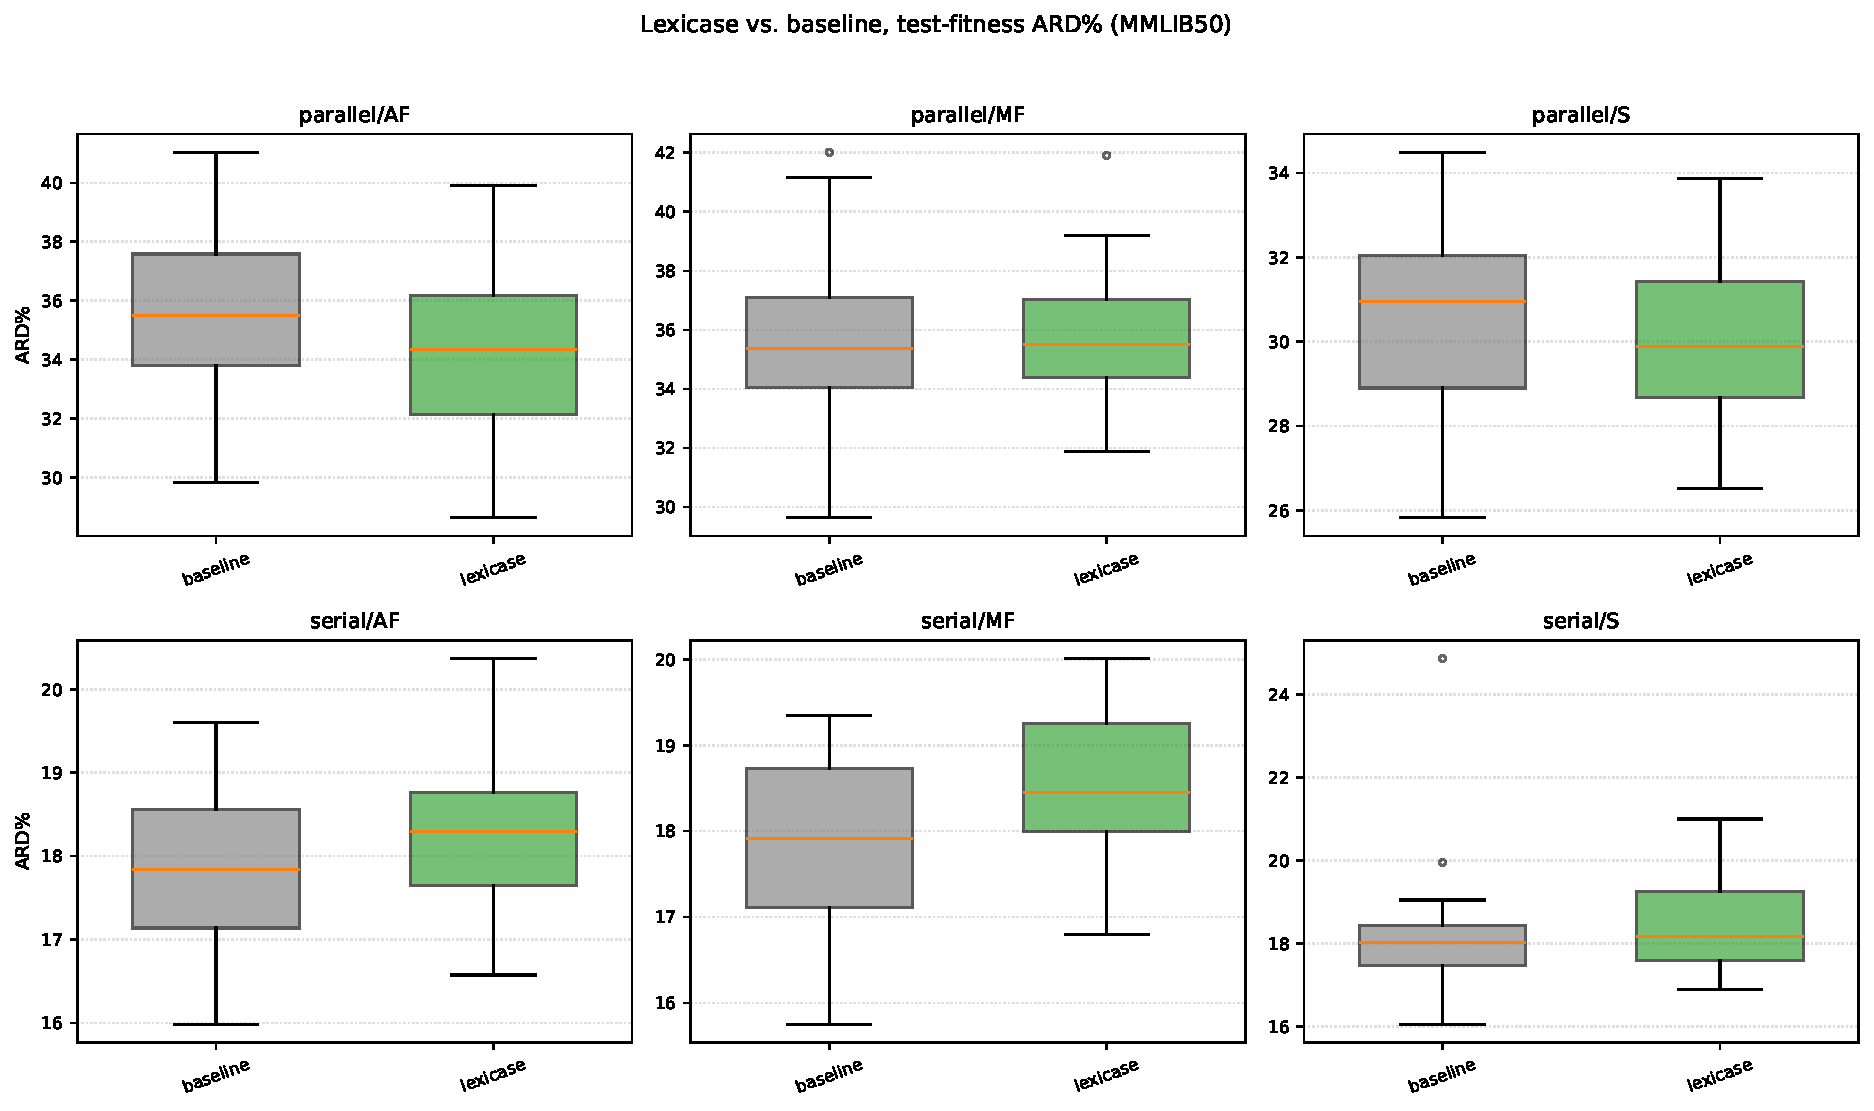
\includegraphics[width=0.95\textwidth]{img/generated/lexicase_boxplot_mmlib50.pdf}
  \caption{Distribution of test-fitness ARD\%, lexicase vs.\ baseline,
  MMLIB50, one panel per (SGS, strategy) cell, 30 seeds per box. Generated
  directly from the raw per-seed result files by
  \texttt{yuantian/experiments/generate\_thesis\_plots.py}.}
  \label{fig:lexicase-boxplot}
\end{figure}

\begin{figure}[htbp]
  \centering
  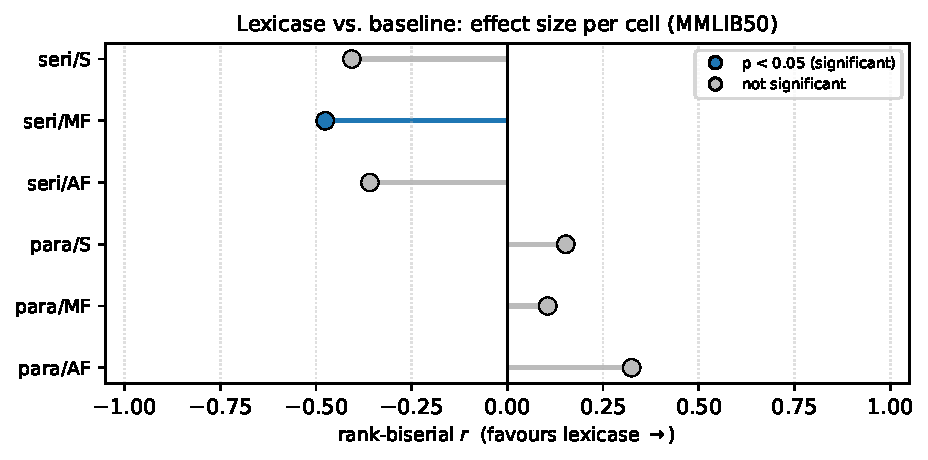
\includegraphics[width=0.85\textwidth]{img/generated/lexicase_effectsize_mmlib50.pdf}
  \caption[Effect-size summary, lexicase vs.\ baseline]{Effect-size summary,
  lexicase vs.\ baseline, MMLIB50: matched rank-biserial correlation $r$ per
  (SGS, strategy) cell (positive favours lexicase), filled markers denote
  $p<0.05$. A full critical-difference diagram is not drawn for this
  two-condition comparison, since with only two conditions the Nemenyi
  post-hoc a CD diagram relies on degenerates to the paired Wilcoxon test
  already reported in Table~\ref{tab:lexicase-significance}; this per-cell
  effect-size view is the more informative visual summary for $k=2$.}
  \label{fig:lexicase-cd}
\end{figure}

\begin{table}[htbp]
  \centering
  \small
  \shrinktofit{%
  \caption[Lexicase vs.\ baseline on MMLIB100]{Mean ARD\% (\%), baseline
  vs.\ epsilon-lexicase selection, MMLIB100 (scalability validation),
  $n=30$ seeds per cell.}
  \label{tab:lexicase-vs-baseline-mmlib100}
  \begin{tabular}{llrrrr}
    \toprule
    \textbf{SGS} & \textbf{Strategy} & \textbf{Baseline (test)} & \textbf{Lexicase (test)} & \textbf{Baseline (train)} & \textbf{Lexicase (train)} \\
    \midrule
    Parallel & AF & 25.40 & 26.24\,\ArrWorse & 19.21 & 20.18\,\ArrWorse \\
    Parallel & MF & 28.04 & 28.00\,\ArrBetter & 20.75 & 20.82\,\ArrWorse \\
    Parallel & S  & 23.28 & 22.76\,\ArrBetter & 16.55 & 16.43\,\ArrBetter \\
    Serial   & AF & 14.64 & 15.37\,\ArrWorse & 12.38 & 12.00\,\ArrBetter \\
    Serial   & MF & 14.88 & 15.39\,\ArrWorse & 12.42 & 11.95\,\ArrBetter \\
    Serial   & S  & 14.68 & 14.38\,\ArrBetter & 12.58 & 12.30\,\ArrBetter \\
    \bottomrule
  \end{tabular}%
  }
\end{table}

\begin{table}[htbp]
  \centering
  \small
  \shrinktofit{%
  \caption[Statistical significance: lexicase vs.\ baseline, MMLIB100]{Two-sided
  paired Wilcoxon signed-rank test and matched rank-biserial effect size
  $r$, lexicase vs.\ baseline, MMLIB100.}
  \label{tab:lexicase-significance-mmlib100}
  \begin{tabular}{lllrrl}
    \toprule
    \textbf{SGS} & \textbf{Strategy} & \textbf{Split} & \textbf{$p$} & \textbf{$r$} & \textbf{Verdict} \\
    \midrule
    Parallel & AF & Train & 0.0000 & $-0.966$ & Significant, favours baseline \\
    Parallel & AF & Test  & 0.0523 & $-0.406$ & Not significant (borderline, favours baseline) \\
    Parallel & MF & Train & 0.3818 & $-0.187$ & Not significant \\
    Parallel & MF & Test  & 0.5291 & $+0.135$ & Not significant \\
    Parallel & S  & Train & 0.2621 & $+0.239$ & Not significant \\
    Parallel & S  & Test  & 0.1909 & $+0.277$ & Not significant \\
    Serial   & AF & Train & 0.0001 & $+0.776$ & Significant, favours lexicase \\
    Serial   & AF & Test  & 0.0054 & $-0.570$ & Significant, favours baseline \\
    Serial   & MF & Train & 0.0000 & $+0.854$ & Significant, favours lexicase \\
    Serial   & MF & Test  & 0.0427 & $-0.424$ & Significant, favours baseline \\
    Serial   & S  & Train & 0.0010 & $+0.665$ & Significant, favours lexicase \\
    Serial   & S  & Test  & 0.1909 & $+0.277$ & Not significant \\
    \bottomrule
  \end{tabular}%
  }
\end{table}

\begin{figure}[htbp]
  \centering
  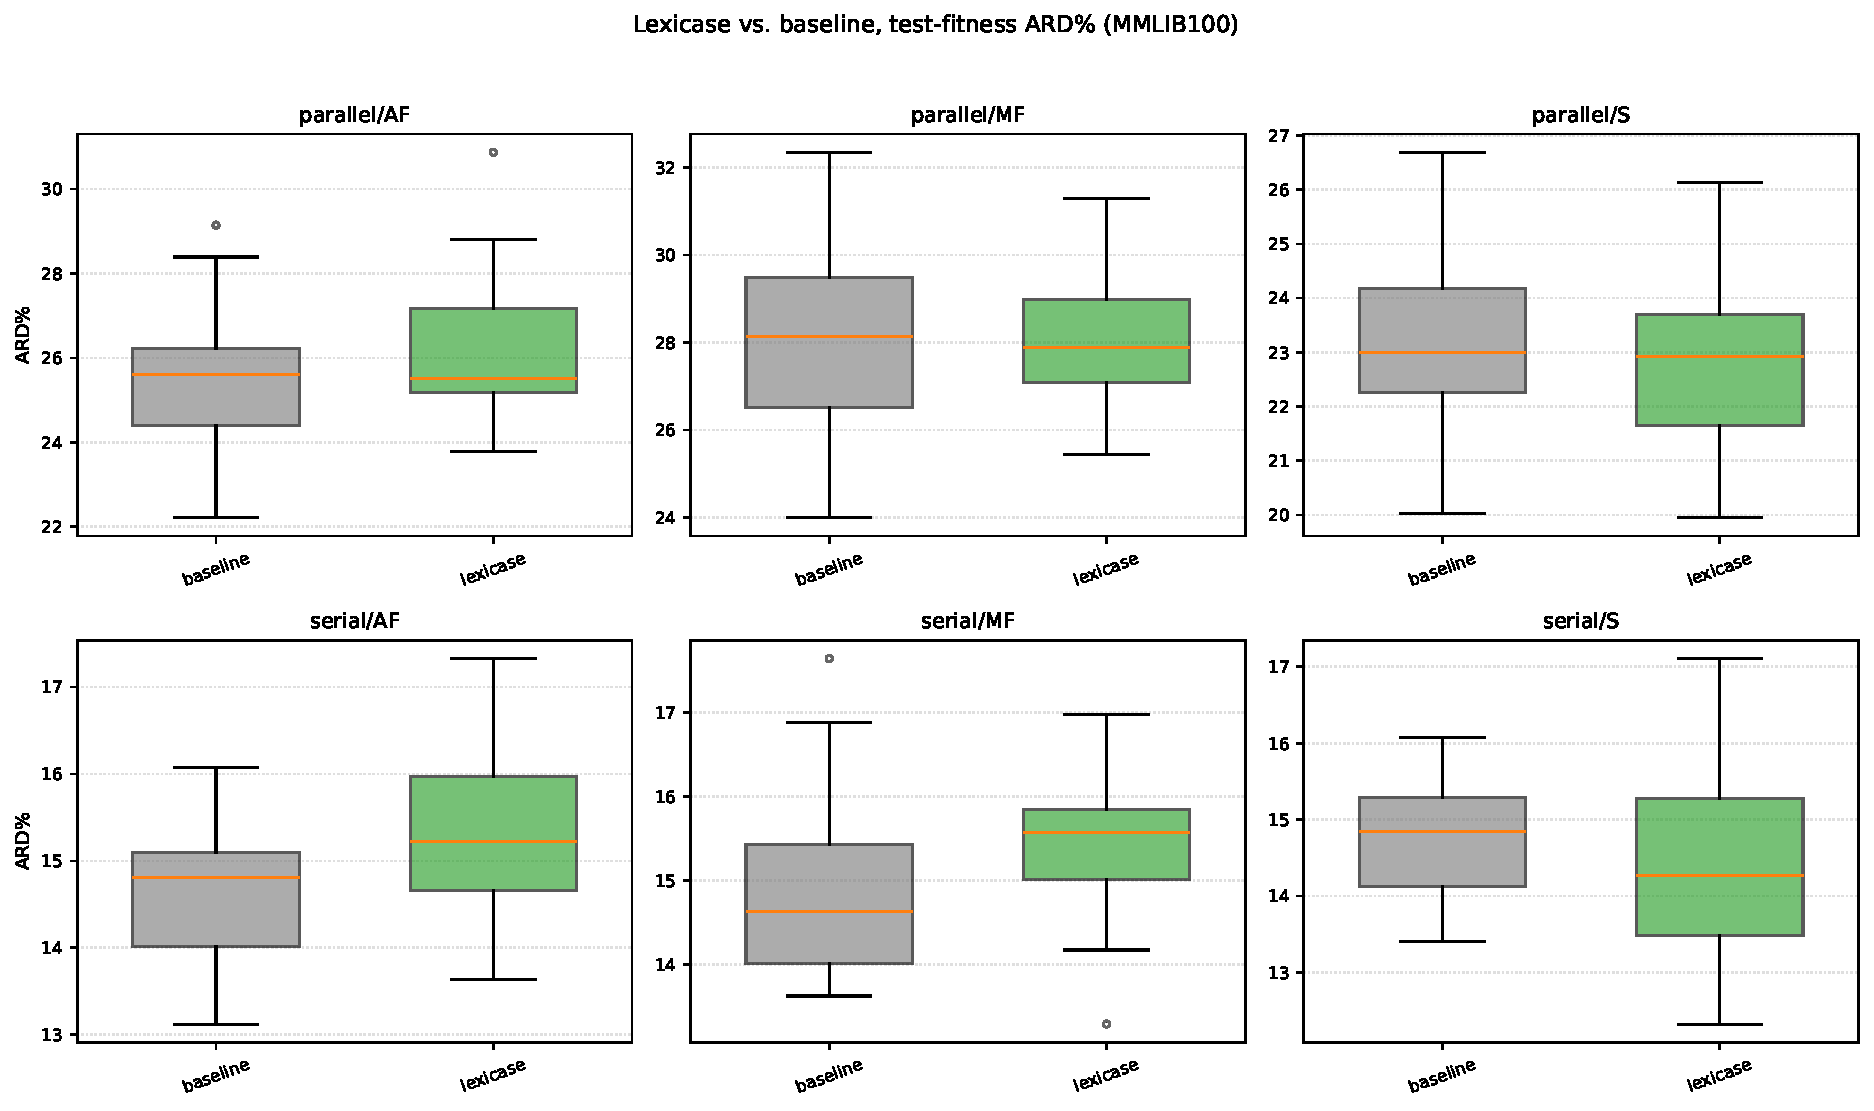
\includegraphics[width=0.95\textwidth]{img/generated/lexicase_boxplot_mmlib100.pdf}
  \caption{Distribution of test-fitness ARD\%, lexicase vs.\ baseline,
  MMLIB100, same layout as Figure~\ref{fig:lexicase-boxplot}.}
  \label{fig:lexicase-boxplot-mmlib100}
\end{figure}

\begin{figure}[htbp]
  \centering
  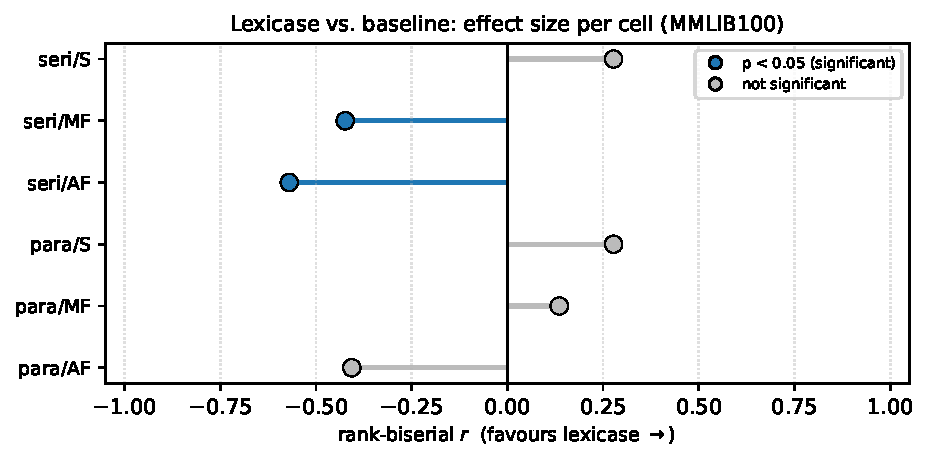
\includegraphics[width=0.85\textwidth]{img/generated/lexicase_effectsize_mmlib100.pdf}
  \caption[Effect-size summary, lexicase vs.\ baseline, MMLIB100]{Effect-size
  summary, lexicase vs.\ baseline, MMLIB100: compare against
  Figure~\ref{fig:lexicase-cd}'s MMLIB50 panel to see the serial-SGS cells
  shift further into unfavourable territory at the larger scale.}
  \label{fig:lexicase-cd-mmlib100}
\end{figure}

\changed{The fully powered comparison confirms, and considerably sharpens,
the pilot's qualitative finding.} On
\emph{training} fitness, lexicase selection shows a clear and consistent,
but direction-dependent, effect: under serial SGS it significantly
outperforms the baseline in all three decision strategies (activity-first
$p=0.0030$, $r=0.604$; mode-first $p=0.0248$, $r=0.467$; simultaneous
$p<0.0001$, $r=0.888$), while under parallel SGS it significantly
\emph{underperforms} the baseline in two of three strategies
(activity-first $p=0.0113$, mode-first $p=0.0327$, both favouring the
baseline). On \emph{test} fitness, \changed{the results} change again: the serial
advantage that was so clear on training data does not reliably survive the
generalisation step, one serial cell (mode-first) reverses into a
significant loss ($p=0.0252$, $r=-0.476$), a second (simultaneous) is a
borderline, non-significant loss ($p=0.0519$), and only the parallel cells
retain a (non-significant) direction favourable to lexicase. Averaged
across all six cells, lexicase's average rank on test fitness (2.33) ties
exactly with the baseline's own (2.33), well behind local search's 1.50
(Section~\ref{subsec:final-comparison}).

\changed{This is a more nuanced result than either the pilot screen or the
original motivation for trying lexicase selection anticipated.} Lexicase
selection reliably finds
GP trees that fit the specific training instances better, an effect large
and consistent enough, under serial SGS especially, to leave little doubt
that the mechanism is doing something real to the search. That advantage,
however, does not transfer reliably to the held-out test instances, and
under serial SGS it can reverse outright. \changed{In practical terms, the
two selection mechanisms are good at different goals: lexicase selection
is the better choice when the aim is to solve a fixed, known set of
instances as well as possible, which is exactly what training fitness
measures, whereas the goal pursued by a hyper-heuristic is a rule that
generalises to unseen instances, so the improvement must appear on the
test data, and there the tournament baseline remains at least as good.} A plausible reading is mild
overfitting: lexicase's case-by-case elimination rewards individuals that
handle the specific quirks of the 30 training instances well, including
quirks that do not generalise, whereas tournament selection's
aggregate-fitness pressure is, if anything, a coarser, more
generalisation-friendly signal precisely because it cannot fixate on any
single instance. Why this reversal is concentrated in serial SGS and not
parallel SGS is a genuinely open question; a candidate explanation, matched
to what changes about decoding between the two, is discussed in
Section~\ref{subsec:localsearch-eval} and returned to in
Chapter~\ref{chap:conclusion}. \changed{Overall, MMLIB50 does not offer
clean evidence that lexicase selection alone is an unambiguous improvement
over the baseline.}

\textbf{Scalability validation.} Table~\ref{tab:lexicase-significance-mmlib100}
answers the question posed above directly: the training-fitness advantage
under serial SGS not only persists at MMLIB100's larger instance size, it
remains significant in all three decision strategies with comparable
effect sizes to MMLIB50 ($r=0.665$--$0.854$, against $r=0.467$--$0.888$ on
MMLIB50). \changed{The test-fitness results, however, do not merely hold
steady, they \emph{sharpen in the unfavourable direction}:} on MMLIB50 only one of
three serial cells reached significance on test fitness (mode-first,
$p=0.0252$); on MMLIB100, two of three do (activity-first, $p=0.0054$,
$r=-0.570$; mode-first, $p=0.0427$, $r=-0.424$), and the third
(simultaneous) sits at a non-significant but still unfavourable-leaning
$r=+0.277$ (a sign flip from MMLIB50's $r=-0.406$, so this one cell alone
does not confirm the pattern). Read together, MMLIB100 strengthens rather
than weakens the mild-overfitting interpretation offered \changed{above}: a larger
instance size did not give lexicase's serial-SGS training advantage more
room to generalise, if anything the training/test gap widened. This is the
clearer of this chapter's two scalability findings: MMLIB100 does not just
fail to overturn the MMLIB50 concern about lexicase's generalisation under
serial SGS, it actively corroborates it.

\changedB{For a concrete picture of the priority rules these statistics
summarise, Figure~\ref{fig:lexicase-evolved-tree} shows a compact rule pair
evolved under lexicase selection. Because lexicase changes only the selection
operator and not the terminal set, the evolved trees draw purely on the
standard baseline vocabulary, so, unlike the NR-aware rule of
Figure~\ref{fig:nr-evolved-tree}, no terminal is highlighted: the difference
lexicase makes is in which individuals survive, not in what they can
express.} \changedC{The pair is also readable once its functionally neutral
code is stripped away: in the activity tree, \texttt{LF}\,\%\,\texttt{LF}
(protected division of a terminal by itself) is the constant $1$ and
$\max(\texttt{LF}, \texttt{LF})$ is simply \texttt{LF}, both typical of the
neutral material GP trees accumulate. What remains is driven almost
entirely by the CPM time-window terminals \texttt{LS} and \texttt{LF}:
since the SGS schedules the activity with the \emph{smallest} rule value
(Section~\ref{subsec:sgs}), the rule prefers activities whose
precedence-feasible window closes early, with the $\texttt{TSC}/\texttt{LF}$
term additionally favouring activities with many transitive successors. The
mode tree is a product of \texttt{GRD}, mode duration and average
requirement, so it prefers short modes with light resource demands.}

\begin{figure}[htbp]
  \centering
  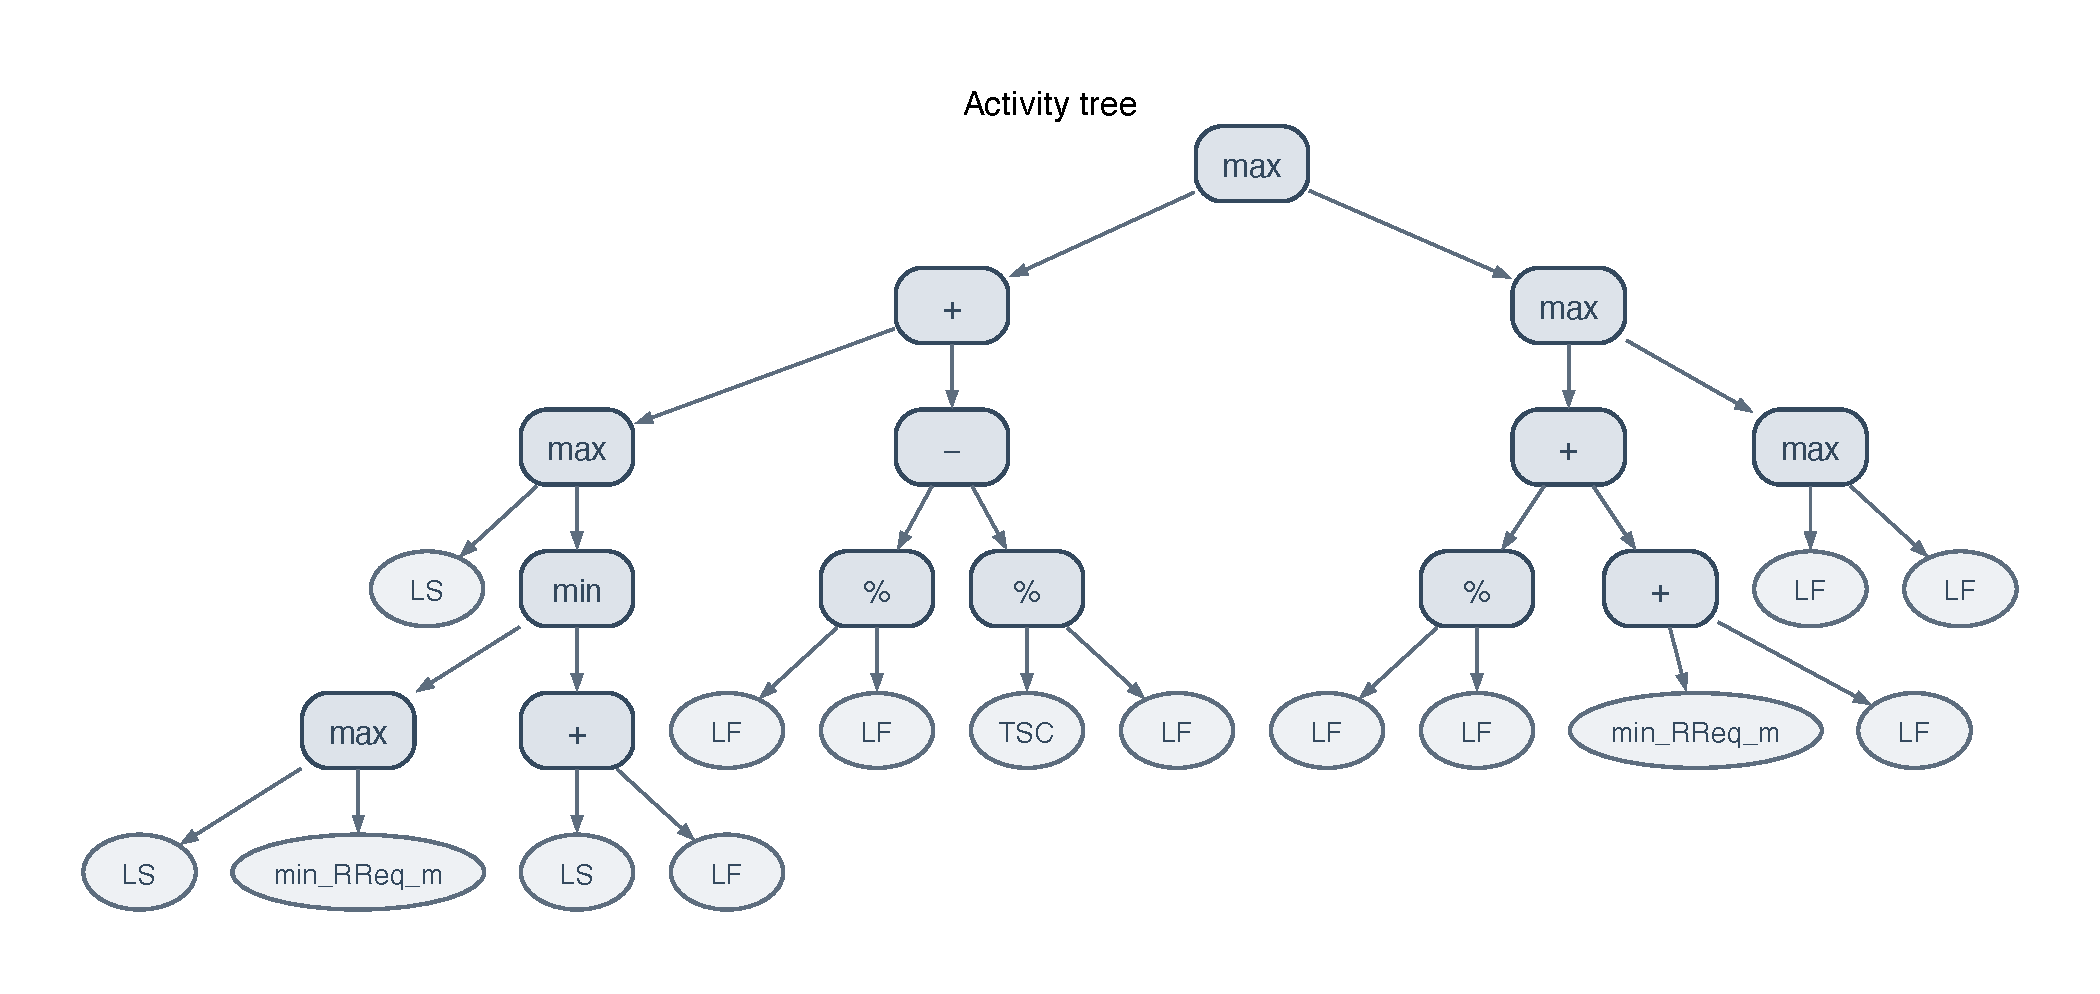
\includegraphics[width=0.98\textwidth]{img/generated/gp_tree_lexicase_activity.pdf}\\[1.5ex]
  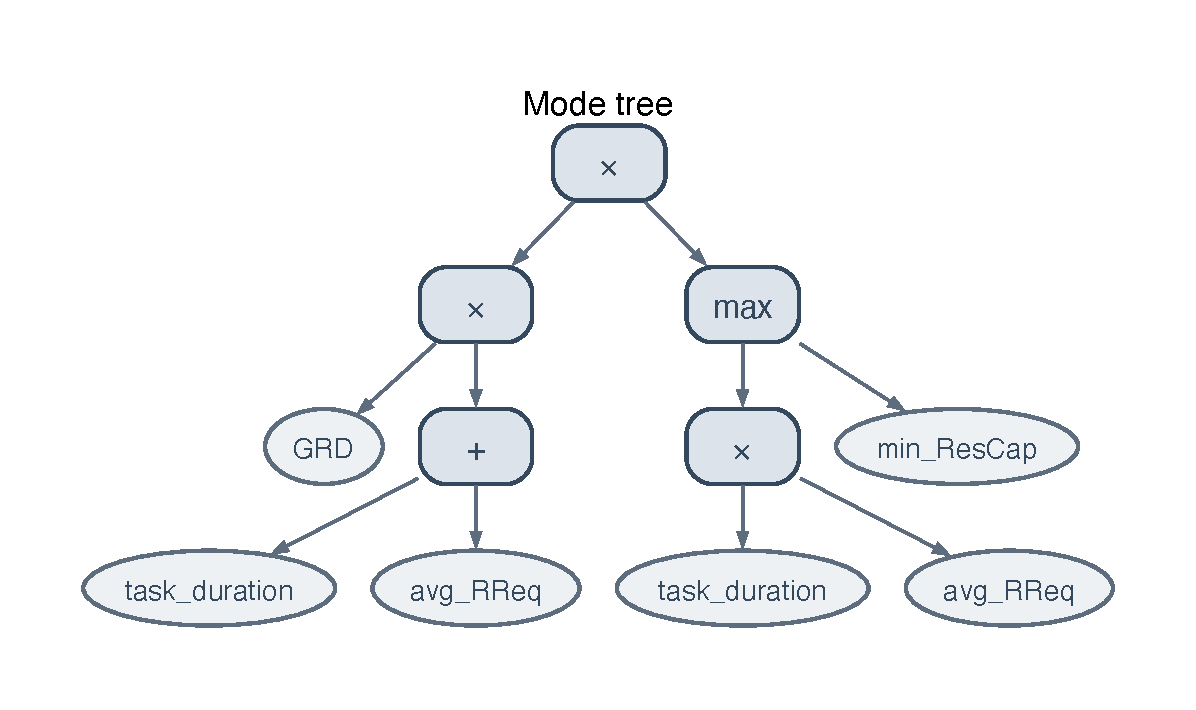
\includegraphics[width=0.5\textwidth]{img/generated/gp_tree_lexicase_mode.pdf}
  \caption[Evolved rule pair under lexicase selection]{\changedB{A compact
  evolved rule pair under lexicase selection (parallel/activity-first,
  MMLIB100), selected as the smallest feasible individual. Top: the activity
  tree; bottom: the mode tree. Operator nodes are blue and terminals grey;
  the standard baseline terminal set is used throughout (no NR terminals).
  Operators as in Figure~\ref{fig:nr-evolved-tree}.}}
  \label{fig:lexicase-evolved-tree}
\end{figure}

\subsection{Comprehensive evaluation of local search with critical path}
\label{subsec:localsearch-eval}

Local search is an attractive complement to a GP-evolved priority rule
because the two operate at different levels: the GP tree decides, in
general, which activity and mode to prefer, while the \changed{Baldwinian}, per-elite
refinement step defined in full in Section~\ref{subsec:localsearch-definition}
can exploit information specific to the one schedule that tree actually
produced on this instance. This section evaluates that mechanism, unchanged,
against the baseline at full statistical power.

\begin{table}[htbp]
  \centering
  \small
  \shrinktofit{%
  \caption[Local search vs.\ baseline on MMLIB50]{Mean ARD\% (\%), baseline
  vs.\ critical-path local search, MMLIB50, $n=30$ seeds per cell.}
  \label{tab:localsearch-vs-baseline-mmlib50}
  \begin{tabular}{llrrrr}
    \toprule
    \textbf{SGS} & \textbf{Strategy} & \textbf{Baseline (test)} & \textbf{Local search (test)} & \textbf{Baseline (train)} & \textbf{Local search (train)} \\
    \midrule
    Parallel & AF & 35.77 & 33.64\,\ArrBetter & 15.94 & 15.72\,\ArrBetter \\
    Parallel & MF & 35.78 & 35.57\,\ArrBetter & 16.61 & 16.87\,\ArrWorse \\
    Parallel & S  & 30.43 & 29.79\,\ArrBetter & 14.20 & 13.95\,\ArrBetter \\
    Serial   & AF & 17.81 & 18.24\,\ArrWorse &  9.83 &  9.85\,\ArrWorse \\
    Serial   & MF & 17.89 & 18.37\,\ArrWorse &  9.82 &  9.87\,\ArrWorse \\
    Serial   & S  & 18.08 & 17.77\,\ArrBetter & 10.29 & 10.29\,\ArrSame \\
    \bottomrule
  \end{tabular}%
  }
\end{table}

\begin{table}[htbp]
  \centering
  \small
  \shrinktofit{%
  \caption[Descriptive statistics: local search vs.\ baseline]{Standard
  deviation accompanying Table~\ref{tab:localsearch-vs-baseline-mmlib50}.
  Feasibility rate is 1.00 for both conditions in every cell.}
  \label{tab:localsearch-descriptive-stats}
  \begin{tabular}{lllrr}
    \toprule
    \textbf{SGS} & \textbf{Strategy} & \textbf{Split} & \textbf{Baseline std} & \textbf{Local search std} \\
    \midrule
    Parallel & AF & Train & 0.58 & 0.55 \\
    Parallel & AF & Test  & 2.74 & 2.61 \\
    Parallel & MF & Train & 0.66 & 0.70 \\
    Parallel & MF & Test  & 2.77 & 2.41 \\
    Parallel & S  & Train & 0.64 & 0.57 \\
    Parallel & S  & Test  & 2.24 & 2.34 \\
    Serial   & AF & Train & 0.25 & 0.25 \\
    Serial   & AF & Test  & 0.91 & 0.91 \\
    Serial   & MF & Train & 0.26 & 0.25 \\
    Serial   & MF & Test  & 0.91 & 0.94 \\
    Serial   & S  & Train & 0.24 & 0.23 \\
    Serial   & S  & Test  & 1.51 & 0.74 \\
    \bottomrule
  \end{tabular}%
  }
\end{table}

\begin{table}[htbp]
  \centering
  \small
  \shrinktofit{%
  \caption[Statistical significance: local search vs.\ baseline]{Two-sided
  paired Wilcoxon signed-rank test and matched rank-biserial effect size
  $r$ (positive favours local search), local search vs.\ baseline, MMLIB50,
  $n=30$ per cell.}
  \label{tab:localsearch-significance}
  \begin{tabular}{lllrrl}
    \toprule
    \textbf{SGS} & \textbf{Strategy} & \textbf{Split} & \textbf{$p$} & \textbf{$r$} & \textbf{Verdict} \\
    \midrule
    Parallel & AF & Train & 0.0803 & $+0.368$ & Not significant \\
    Parallel & AF & Test  & 0.0026 & $+0.613$ & Significant, favours local search \\
    Parallel & MF & Train & 0.1191 & $-0.329$ & Not significant \\
    Parallel & MF & Test  & 0.9677 & $+0.011$ & Not significant \\
    Parallel & S  & Train & 0.1241 & $+0.325$ & Not significant \\
    Parallel & S  & Test  & 0.1981 & $+0.273$ & Not significant \\
    Serial   & AF & Train & 0.8553 & $-0.041$ & Not significant \\
    Serial   & AF & Test  & 0.1274 & $-0.324$ & Not significant \\
    Serial   & MF & Train & 0.4645 & $-0.157$ & Not significant \\
    Serial   & MF & Test  & 0.0961 & $-0.351$ & Not significant \\
    Serial   & S  & Train & 0.8078 & $+0.054$ & Not significant \\
    Serial   & S  & Test  & 0.6263 & $+0.105$ & Not significant \\
    \bottomrule
  \end{tabular}%
  }
\end{table}

\begin{figure}[htbp]
  \centering
  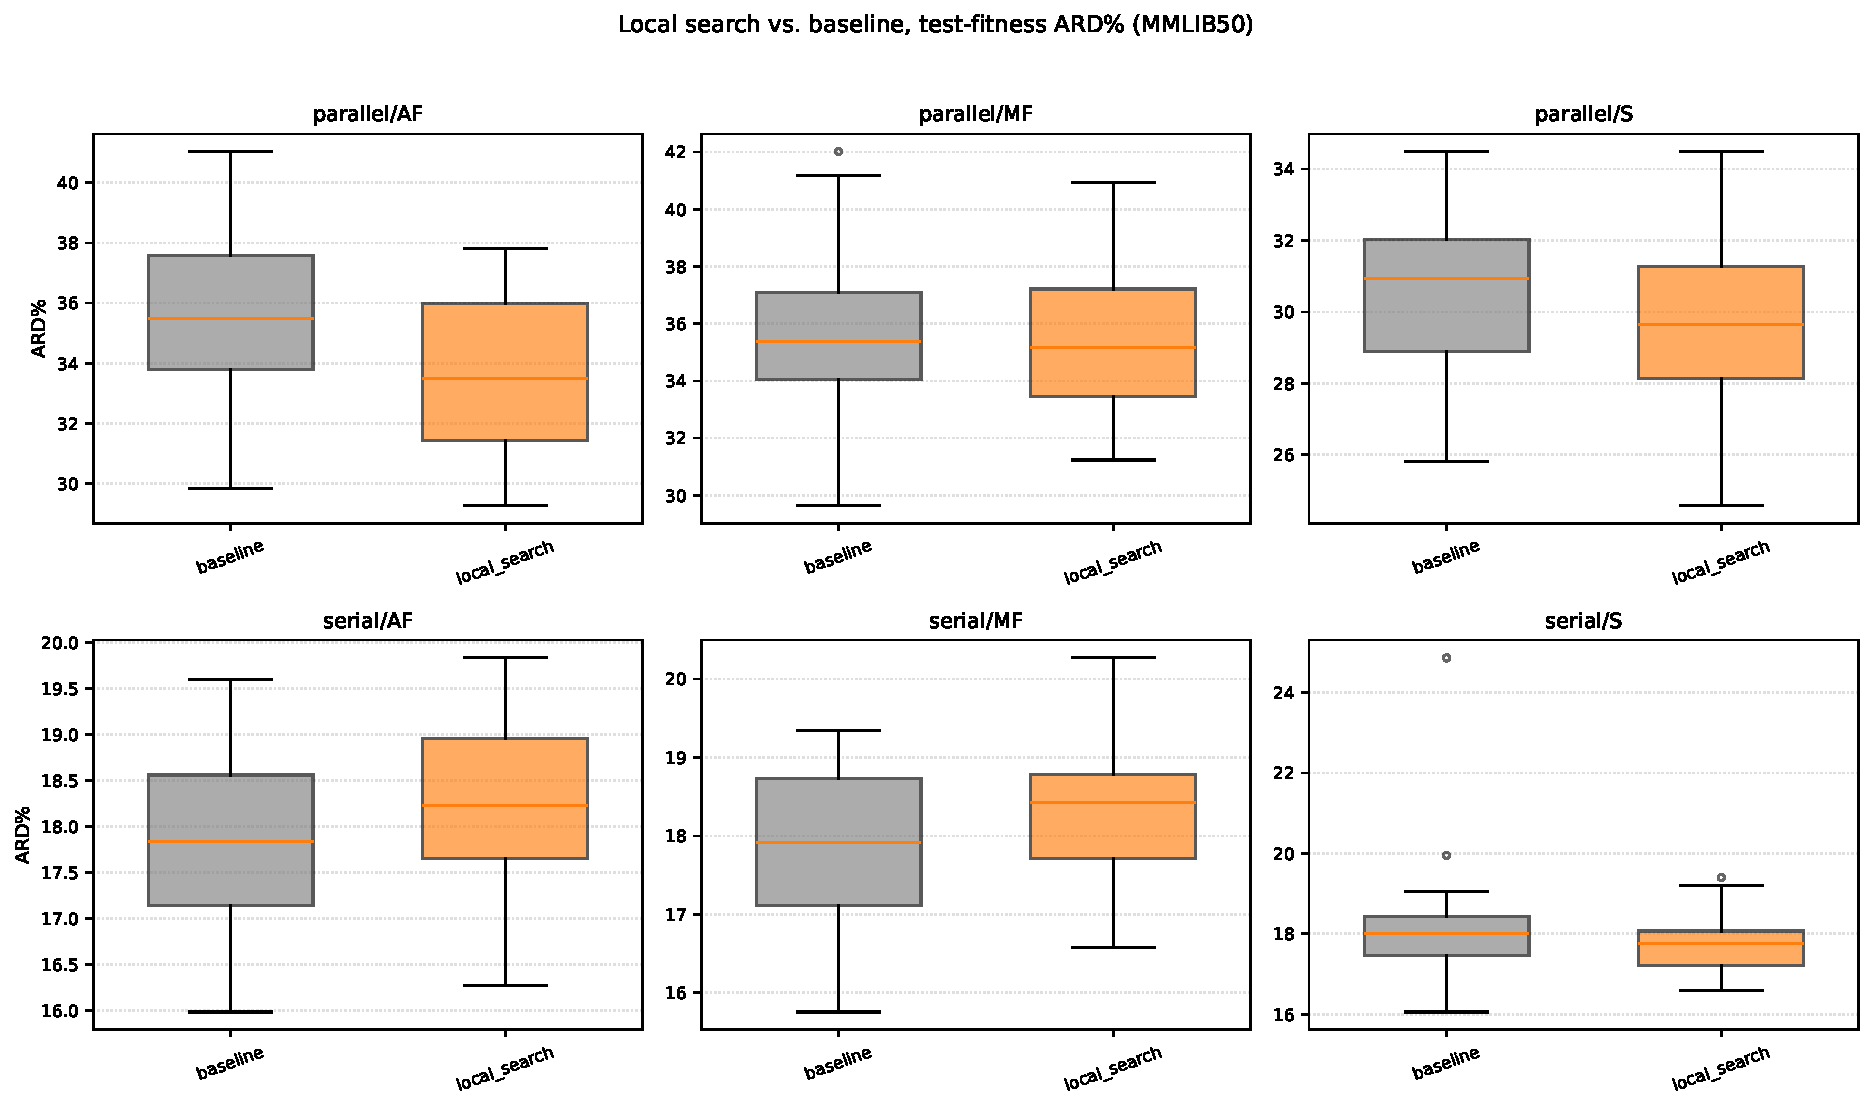
\includegraphics[width=0.95\textwidth]{img/generated/localsearch_boxplot_mmlib50.pdf}
  \caption{Distribution of test-fitness ARD\%, local search vs.\ baseline,
  MMLIB50, one panel per (SGS, strategy) cell, 30 seeds per box.}
  \label{fig:localsearch-boxplot}
\end{figure}

\begin{figure}[htbp]
  \centering
  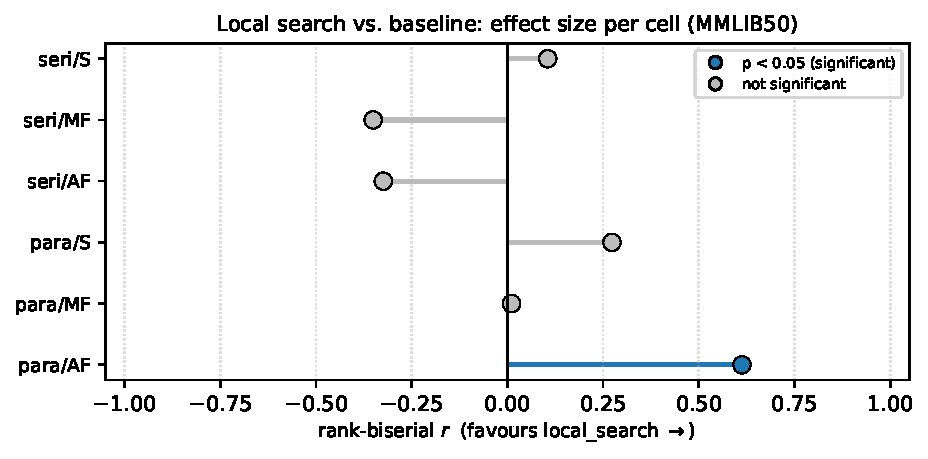
\includegraphics[width=0.85\textwidth]{img/generated/localsearch_effectsize_mmlib50.pdf}
  \caption[Effect-size summary, local search vs.\ baseline]{Effect-size
  summary, local search vs.\ baseline, MMLIB50: matched rank-biserial
  correlation $r$ per (SGS, strategy) cell (positive favours local search),
  filled markers denote $p<0.05$; see Figure~\ref{fig:lexicase-cd}'s caption
  for why a per-cell effect-size plot, not a Nemenyi CD diagram, is used for
  this two-condition comparison.}
  \label{fig:localsearch-cd}
\end{figure}

\begin{table}[htbp]
  \centering
  \small
  \shrinktofit{%
  \caption[Local search vs.\ baseline on MMLIB100]{Mean ARD\% (\%), baseline
  vs.\ critical-path local search, MMLIB100 (scalability validation), $n=30$
  seeds per cell.}
  \label{tab:localsearch-vs-baseline-mmlib100}
  \begin{tabular}{llrrrr}
    \toprule
    \textbf{SGS} & \textbf{Strategy} & \textbf{Baseline (test)} & \textbf{Local search (test)} & \textbf{Baseline (train)} & \textbf{Local search (train)} \\
    \midrule
    Parallel & AF & 25.40 & 25.90\,\ArrWorse & 19.21 & 19.45\,\ArrWorse \\
    Parallel & MF & 28.04 & 28.40\,\ArrWorse & 20.75 & 21.01\,\ArrWorse \\
    Parallel & S  & 23.28 & 23.60\,\ArrWorse & 16.55 & 16.79\,\ArrWorse \\
    Serial   & AF & 14.64 & 14.71\,\ArrWorse & 12.38 & 12.38\,\ArrSame \\
    Serial   & MF & 14.88 & 14.78\,\ArrBetter & 12.42 & 12.35\,\ArrBetter \\
    Serial   & S  & 14.68 & 14.68\,\ArrSame & 12.58 & 12.75\,\ArrWorse \\
    \bottomrule
  \end{tabular}%
  }
\end{table}

\begin{table}[htbp]
  \centering
  \small
  \shrinktofit{%
  \caption[Statistical significance: local search vs.\ baseline, MMLIB100]{Two-sided
  paired Wilcoxon signed-rank test and matched rank-biserial effect size
  $r$, local search vs.\ baseline, MMLIB100.}
  \label{tab:localsearch-significance-mmlib100}
  \begin{tabular}{lllrrl}
    \toprule
    \textbf{SGS} & \textbf{Strategy} & \textbf{Split} & \textbf{$p$} & \textbf{$r$} & \textbf{Verdict} \\
    \midrule
    Parallel & AF & Train & 0.3285 & $-0.209$ & Not significant \\
    Parallel & AF & Test  & 0.2621 & $-0.239$ & Not significant \\
    Parallel & MF & Train & 0.0699 & $-0.381$ & Not significant \\
    Parallel & MF & Test  & 0.2367 & $-0.252$ & Not significant \\
    Parallel & S  & Train & 0.2286 & $-0.256$ & Not significant \\
    Parallel & S  & Test  & 0.5561 & $-0.127$ & Not significant \\
    Serial   & AF & Train & 0.7000 & $-0.084$ & Not significant \\
    Serial   & AF & Test  & 0.8872 & $-0.032$ & Not significant \\
    Serial   & MF & Train & 0.5158 & $+0.140$ & Not significant \\
    Serial   & MF & Test  & 0.9193 & $+0.024$ & Not significant \\
    Serial   & S  & Train & 0.0803 & $-0.368$ & Not significant \\
    Serial   & S  & Test  & 0.8022 & $+0.054$ & Not significant \\
    \bottomrule
  \end{tabular}%
  }
\end{table}

\begin{figure}[htbp]
  \centering
  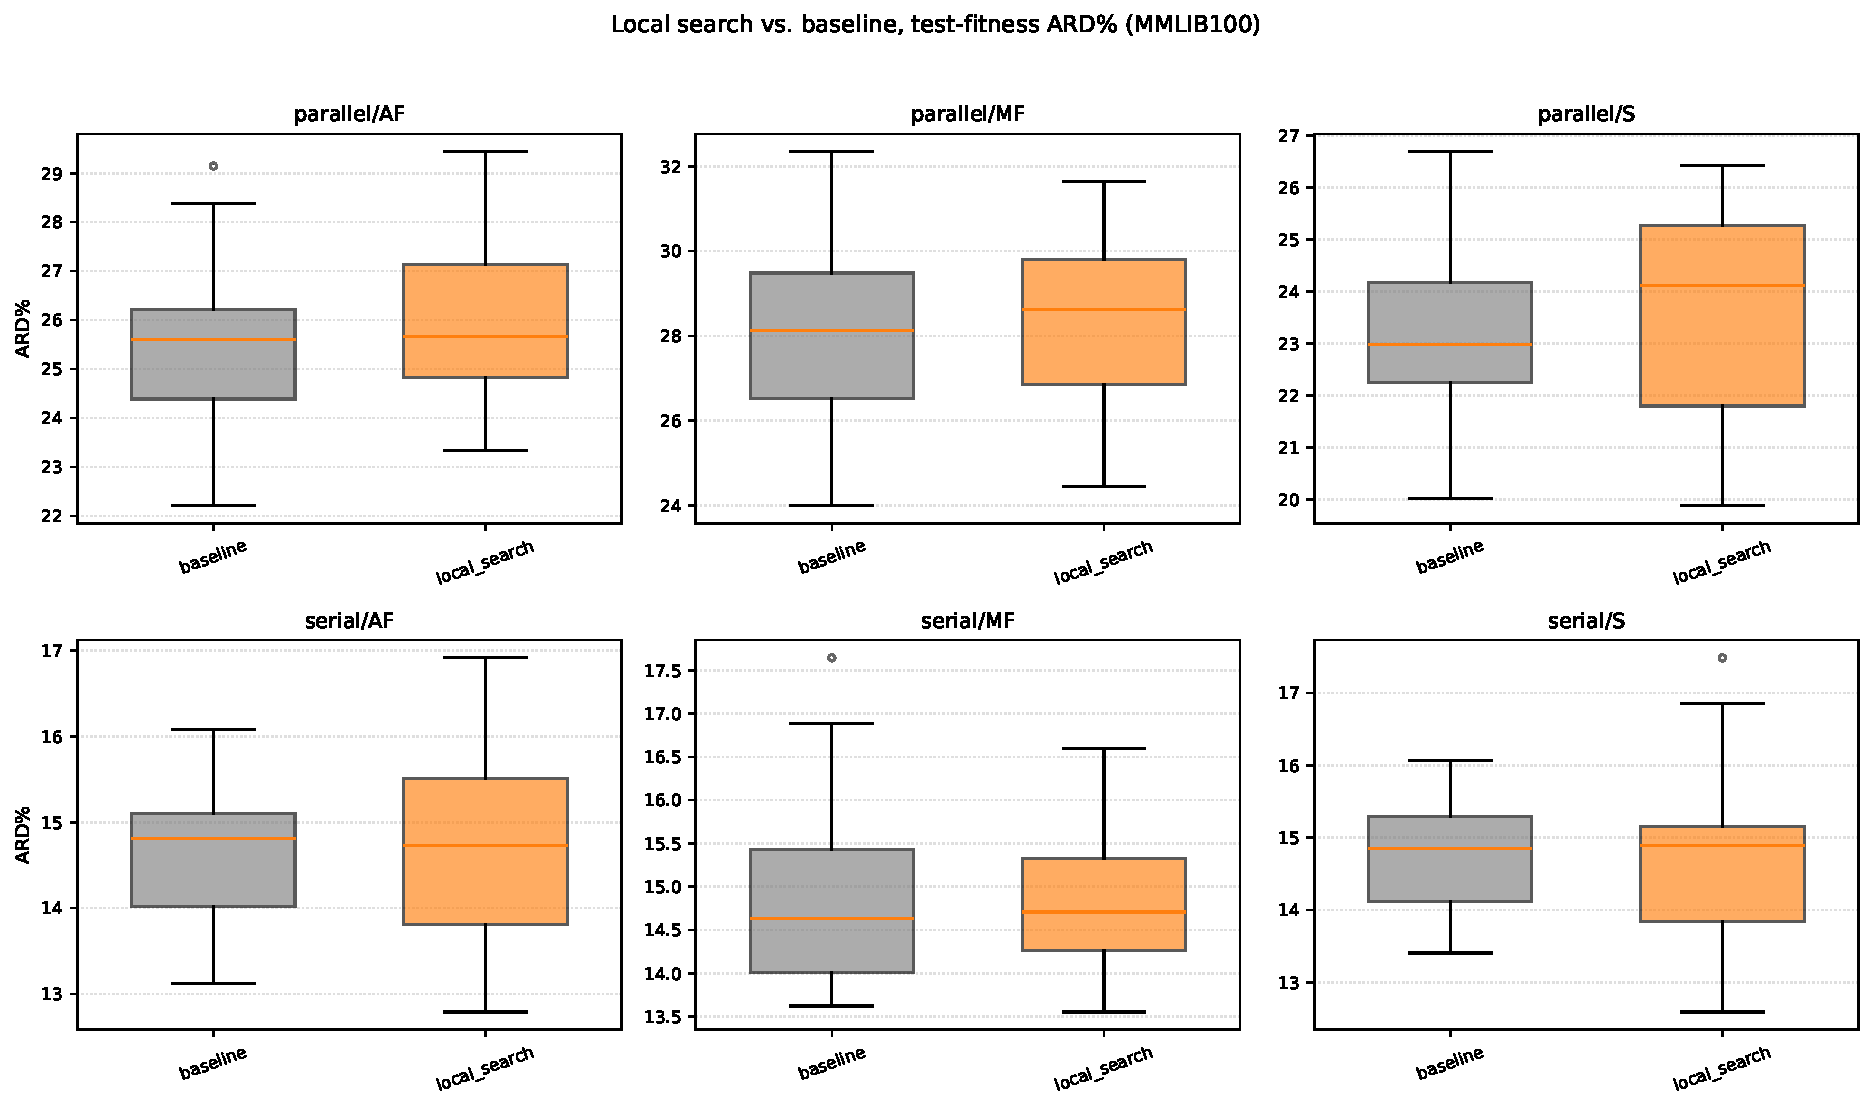
\includegraphics[width=0.95\textwidth]{img/generated/localsearch_boxplot_mmlib100.pdf}
  \caption{Distribution of test-fitness ARD\%, local search vs.\ baseline,
  MMLIB100, same layout as Figure~\ref{fig:localsearch-boxplot}.}
  \label{fig:localsearch-boxplot-mmlib100}
\end{figure}

\begin{figure}[htbp]
  \centering
  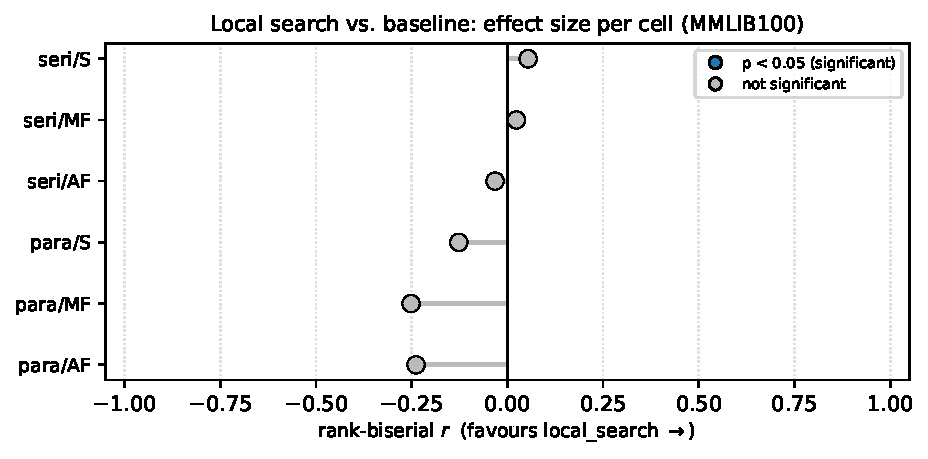
\includegraphics[width=0.85\textwidth]{img/generated/localsearch_effectsize_mmlib100.pdf}
  \caption[Effect-size summary, local search vs.\ baseline, MMLIB100]{Effect-size
  summary, local search vs.\ baseline, MMLIB100: every cell sits much closer
  to zero than its MMLIB50 counterpart in Figure~\ref{fig:localsearch-cd},
  visualising the loss of the one significant MMLIB50 win.}
  \label{fig:localsearch-cd-mmlib100}
\end{figure}

Table~\ref{tab:localsearch-significance} tells a more qualified story than
the section's motivation might suggest. Exactly one of the twelve
train/test comparisons reaches significance: parallel/activity-first test
fitness improves from 35.77\% to 33.64\% ($p=0.0026$, $r=0.613$, a
moderately large effect). No other cell, train or test, serial or parallel,
reaches conventional significance, and the \emph{direction} of the
(non-significant) effect itself depends systematically on SGS: all three
parallel test cells favour local search (activity-first significantly so,
mode-first and simultaneous non-significantly), while two of the three
serial test cells favour the baseline instead. Averaged across all six
cells, local search nonetheless achieves the best average test-fitness rank
of any of the four directly comparable conditions (1.50, ahead of baseline
and lexicase at 2.33 each and hybrid at 3.83,
Section~\ref{subsec:final-comparison}), driven by consistently
favourable, even if individually non-significant, performance under
parallel SGS.

A plausible explanation for this SGS-dependent pattern lies in how much
room each decoding scheme leaves for a post-hoc, per-instance refinement
step to exploit. Parallel SGS advances a single global clock and commits
several activities to the same time step at once, which tends to leave more
slack, and more genuinely improvable local structure, in the resulting
schedule for the resource-shift move to find and exploit. Serial SGS's
greedy, one-activity-at-a-time construction already resolves many of the
same local trade-offs as it builds the schedule, leaving comparatively
little for a subsequent hill-climb to improve on, and occasionally
disturbing a schedule that was already close to locally optimal for that
decoding scheme. This reading is consistent with, and offers one candidate
explanation for, Section~\ref{subsec:lexicase-eval}'s otherwise puzzling
observation that lexicase's train/test gap was also concentrated in serial
SGS: if serial-SGS schedules are, in this sense, closer to a local optimum
of the decoding scheme itself, then a training-fitness gain obtained
against them (whether via selection or via local search) may more often
represent fitting to idiosyncrasies of the specific training instances
rather than a generalisable improvement in the underlying priority rule.
Confirming this would require directly instrumenting the local search's
accepted-move statistics per SGS, which was not done for this thesis and is
noted as future work (Section~\ref{sec:future-work}).

\changed{In summary, the result is more measured than the mechanism's
motivation promised.} The mechanism is
sound, produces one clearly significant, moderately sized improvement, and
its overall effect direction is favourable more often than not; but at this
scale and this evaluation budget, it does not deliver a broad,
strategy-independent improvement over the baseline, and its benefit appears
concentrated in exactly the decoding scheme (parallel) where more
improvable structure remains in the schedule after construction.

\textbf{Scalability validation.} \changed{This finding does \emph{not}
survive scaling up.} Table~\ref{tab:localsearch-significance-mmlib100}
shows \emph{no} significant cell anywhere, train or test, parallel or
serial: MMLIB50's one significant win, parallel/activity-first test fitness
($p=0.0026$, $r=0.613$), is not merely weaker at MMLIB100, it is essentially
absent ($p=0.2621$, $r=-0.239$, now leaning in the \emph{unfavourable}
direction). The parallel-favours-local-search, serial-does-not asymmetry
\changed{that motivated the candidate explanation above} (parallel SGS leaving more exploitable
slack) does partially reappear as a direction, five of six MMLIB100 cells
still lean the same way as their MMLIB50 counterparts, but none of the six
individual comparisons clears significance at this instance size, and the
one comparison that did clear it on MMLIB50 specifically fails to replicate.
\changed{Critical-path local search's MMLIB50 benefit, already the most
narrowly supported of the three comprehensive-stage results, therefore
does not scale cleanly to MMLIB100 in this evaluation, which qualifies its
favourable average rank in the final comparison
(Section~\ref{subsec:final-comparison} returns to this point directly).}

\changedB{As with lexicase, Figure~\ref{fig:localsearch-evolved-tree} gives a
concrete example of a rule pair evolved under the critical-path local search.
The mechanism is Baldwinian: local search improves the schedule an
individual decodes to but leaves its terminal set unchanged, so here too the
evolved trees use only the standard baseline vocabulary and no terminal is
highlighted.} \changedC{The single smallest local-search individual is
uninformative to read: because \texttt{LS} and \texttt{EF} are never
negative, its activity tree collapses to the bare terminal \texttt{LS}, the
classic minimum-\emph{LST} rule, which is sensible in itself (the
activities whose time window closes earliest are scheduled first) but shows
nothing beyond a single terminal.
Figure~\ref{fig:localsearch-evolved-tree} therefore shows, from two
champions of the same serial/mode-first MMLIB100 cell, the most compact
genuinely composite example of each tree type. The activity tree computes
$\min(\texttt{LS},\, \max(\texttt{LS}/\texttt{SC},\,
\texttt{ES} + \texttt{PC}))$ (the duplicated $\max(\texttt{LS},
\texttt{LS})$ \changedD{simplifies to} \texttt{LS}): a latest-start-time rule
at its core, in which an activity with several immediate successors
(\texttt{SC} large, so $\texttt{LS}/\texttt{SC}$ small) and an early
earliest start can score below its own \texttt{LS} and so move forward in
the queue. The mode tree does not collapse to a single terminal either,
but both arguments of its root $\min$ grow with \texttt{EFFT} and
\texttt{RR}, so it consistently prefers modes that can finish early and
request few resource types.}

\changedC{The displayed pairs are hand-picked for compactness, so it is
fair to ask how representative they are of what evolution produces at
large. A check across every comprehensive-stage champion (all 2\,160
best-of-run individuals; script
\texttt{yuantian/experiments/champion\_tree\_analysis.py}, which tests
order-equivalence by sampling random terminal assignments) shows that a
complete collapse to a single terminal, like that of the smallest
local-search individual just described, is rare, roughly $1$--$3\%$ of
two-tree champions per condition, and when it does happen the surviving
terminal is always \texttt{LS} under serial SGS and almost always
\texttt{LF} under parallel SGS. The
vocabulary of the displayed pairs is, however, entirely typical: under
serial SGS practically every champion's activity tree recruits
\texttt{LS} ($99$--$100\%$ across the four renewable-instance
conditions, with \texttt{LF} second at $85$--$88\%$), under parallel SGS
\texttt{LF} leads ($92$--$97\%$), and the mode trees recruit
\texttt{EFFT} universally under serial SGS alongside the resource-demand
aggregates (\texttt{avg\_RReq}, \texttt{GRD}, \texttt{task\_duration}).
What the evolved rules decide by is thus consistent across the
population: CPM time-window terminals rank activities, and early-finish,
low-demand terminals rank modes; the figures differ from the population
only in how little else they carry around that core.}

\begin{figure}[htbp]
  \centering
  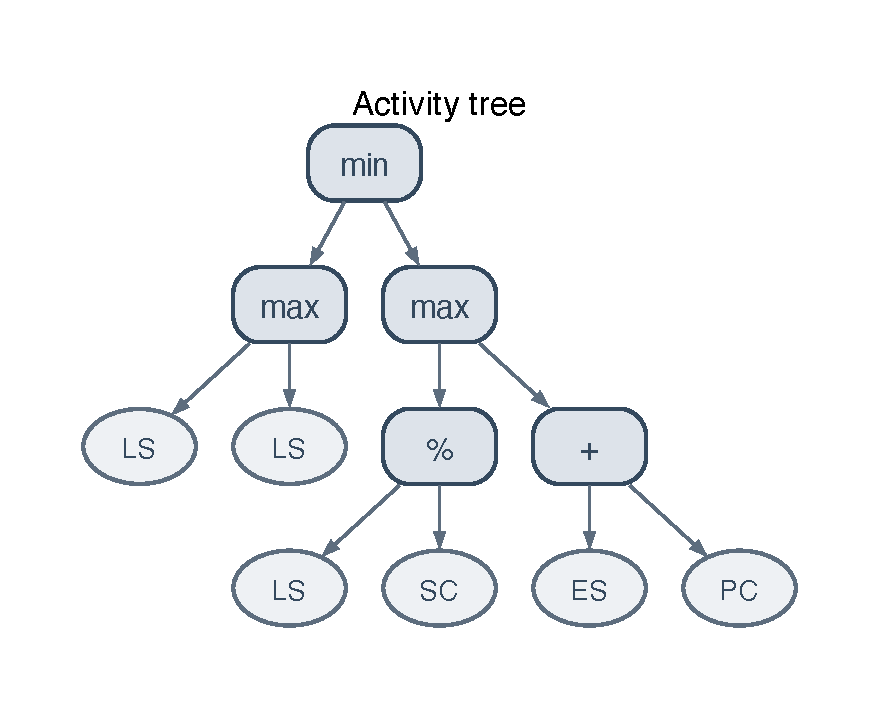
\includegraphics[width=0.5\textwidth]{img/generated/gp_tree_localsearch_activity.pdf}\\[1.5ex]
  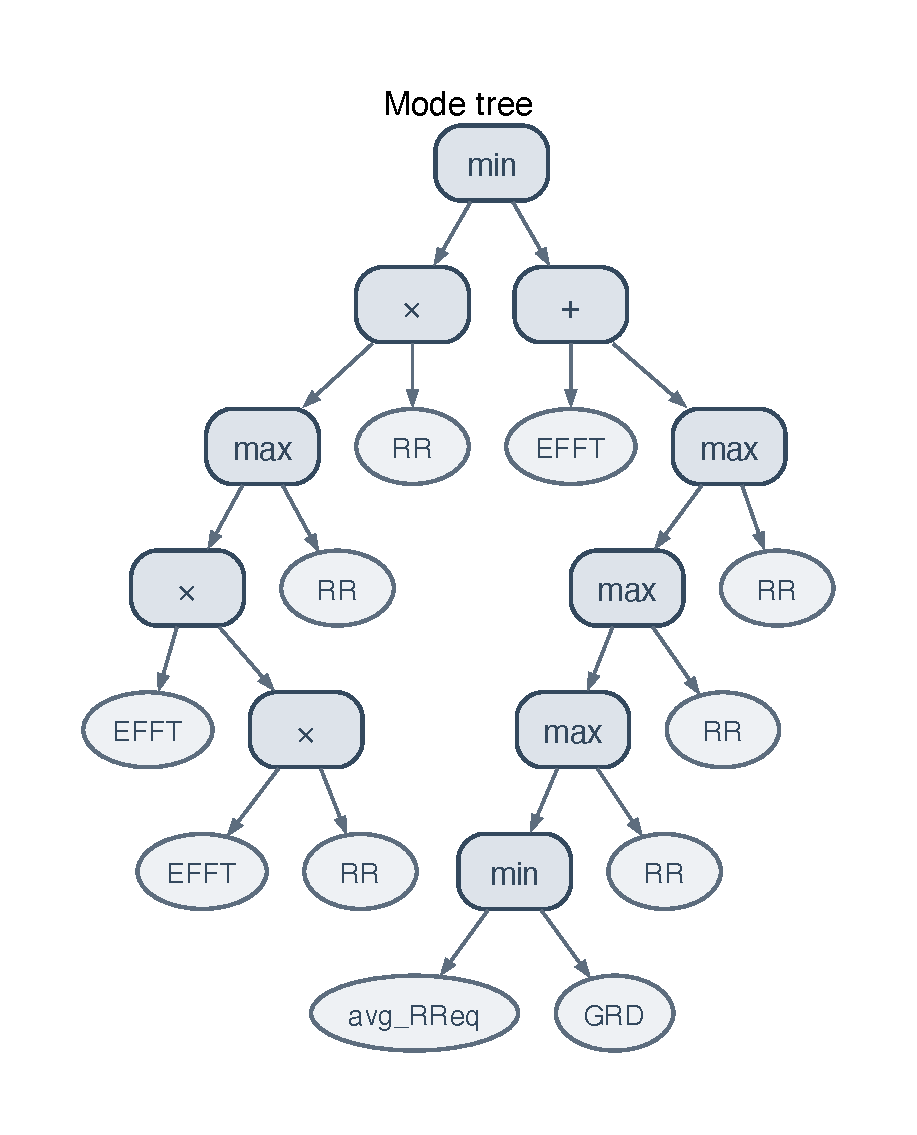
\includegraphics[width=0.78\textwidth]{img/generated/gp_tree_localsearch_mode.pdf}
  \caption[Evolved activity and mode tree under critical-path local
  search]{\changedC{Compact evolved trees under critical-path local search
  (serial/mode-first, MMLIB100). The two panels are from two champions of
  that cell, each chosen as the most compact interpretable example of its
  tree type, since the smallest single individual's activity tree collapses
  to the bare minimum-LST terminal \texttt{LS}. Top: an activity tree,
  $\min(\texttt{LS}, \max(\texttt{LS}/\texttt{SC},
  \texttt{ES} + \texttt{PC}))$, a minimum-latest-start-time rule that lets
  activities with several immediate successors move forward (the duplicated
  $\max(\texttt{LS}, \texttt{LS})$ \changedD{simplifies to} \texttt{LS}).
  Bottom: a mode tree, which prefers modes that finish early (\texttt{EFFT})
  and request few resource types (\texttt{RR}).} \changedB{Colours and
  operators as in Figure~\ref{fig:nr-evolved-tree}; the standard baseline
  terminal set is used throughout.}}
  \label{fig:localsearch-evolved-tree}
\end{figure}

\subsection{Comprehensive evaluation of NR terminals}
\label{subsec:nr-eval}

NR terminals (defined in full in Section~\ref{subsec:nr-terminals-definition}:
\texttt{NR\_STOCK\_RATIO}, \texttt{NR\_MODE\_DEMAND\_RATIO}, and
\texttt{NR\_BUDGET\_PRESSURE}) close the baseline terminal set's one
significant blind spot, visibility into non-renewable resource state, and
are evaluated here for the first time at full statistical power. Because
these terminals are only meaningful on instances that still carry their
non-renewable resources, this condition is evaluated on NR-preserving
instances rather than \changedC{the renewable-only-converted set of the
baseline paper (Tian et al.~\cite{Tian2024GPHH})} used
everywhere else in this chapter, against \texttt{baseline\_nr}, the
unmodified baseline algorithm run on the same NR-preserving instances, as
its matched control. The two conditions are directly comparable to each
other, but their ARD\% figures are \emph{not} comparable in magnitude to
the baseline/lexicase/local-search figures above, because the CPM lower
bound used for normalisation ignores resource constraints entirely
(Section~\ref{sec:eval-metrics}), and is consequently far looser, relative
to true achievable makespan, on NR-preserving instances than on the
renewable-only-converted ones. \changedC{Because infeasible schedules have
no meaningful makespan, every ARD\% figure in the tables of this section
(as everywhere in this chapter,
Section~\ref{subsec:statistical-methodology}) is a mean over the instances
a rule scheduled feasibly; the instances it failed on are not
\changedD{included in} the mean but reported separately, as the feasibility rate in
Table~\ref{tab:nr-descriptive-stats} for MMLIB50 and
Table~\ref{tab:nr-descriptive-stats-mmlib100} for MMLIB100. This matters here more than in the
two comparisons above, where feasibility was uniformly $1.00$: when
conditions differ in feasibility, their feasible-only means are computed
over different instance subsets, which is why the two metrics must always
be read together.}

\begin{table}[htbp]
  \centering
  \small
  \shrinktofit{%
  \caption[NR terminals vs.\ baseline on MMLIB50]{Mean ARD\% (\%),
  \texttt{baseline\_nr} vs.\ NR terminals, MMLIB50 (NR-preserving
  instances), $n=30$ seeds per cell.}
  \label{tab:nr-vs-baseline-mmlib50}
  \begin{tabular}{llrrrr}
    \toprule
    \textbf{SGS} & \textbf{Strategy} & \textbf{\texttt{baseline\_nr} (test)} & \textbf{NR terminals (test)} & \textbf{\texttt{baseline\_nr} (train)} & \textbf{NR terminals (train)} \\
    \midrule
    Parallel & AF & 140.92 & 121.74\,\ArrBetter & 121.89 & 102.99\,\ArrBetter \\
    Parallel & MF & 143.14 & 124.85\,\ArrBetter & 123.11 & 105.66\,\ArrBetter \\
    Parallel & S  & 144.86 & 129.27\,\ArrBetter & 123.27 & 108.49\,\ArrBetter \\
    Serial   & AF & 140.36 & 109.23\,\ArrBetter & 120.86 &  88.10\,\ArrBetter \\
    Serial   & MF & 139.05 & 113.54\,\ArrBetter & 119.86 &  90.13\,\ArrBetter \\
    Serial   & S  & 144.34 & 110.37\,\ArrBetter & 123.71 &  87.41\,\ArrBetter \\
    \bottomrule
  \end{tabular}%
  }
\end{table}

\begin{table}[htbp]
  \centering
  \small
  \shrinktofit{%
  \caption[Descriptive statistics: NR terminals vs.\ baseline]{Standard
  deviation and, unlike the two comparisons above, a clearly
  \emph{non-uniform} feasibility rate: NR terminals raise held-out test
  feasibility from roughly 68--70\% to roughly 82--86\% across every cell,
  in addition to improving the feasible-only mean ARD\% reported in
  Table~\ref{tab:nr-vs-baseline-mmlib50}.}
  \label{tab:nr-descriptive-stats}
  \begin{tabular}{lllrrrr}
    \toprule
    \textbf{SGS} & \textbf{Strategy} & \textbf{Split} & \textbf{\texttt{baseline\_nr} std} & \textbf{NR std} & \textbf{\texttt{baseline\_nr} feas.} & \textbf{NR feas.} \\
    \midrule
    Parallel & AF & Train &  8.60 & 8.61 & 0.93 & 1.00 \\
    Parallel & AF & Test  & 14.84 & 11.69 & 0.69 & 0.85 \\
    Parallel & MF & Train &  6.49 & 5.67 & 0.93 & 1.00 \\
    Parallel & MF & Test  & 10.98 & 9.77 & 0.69 & 0.82 \\
    Parallel & S  & Train &  5.74 & 4.70 & 0.94 & 1.00 \\
    Parallel & S  & Test  &  8.15 & 8.34 & 0.68 & 0.82 \\
    Serial   & AF & Train &  4.76 & 5.47 & 1.00 & 1.00 \\
    Serial   & AF & Test  &  6.05 & 9.77 & 0.69 & 0.82 \\
    Serial   & MF & Train &  7.59 & 6.88 & 1.00 & 1.00 \\
    Serial   & MF & Test  & 13.25 & 8.96 & 0.68 & 0.83 \\
    Serial   & S  & Train &  4.71 & 7.54 & 0.98 & 1.00 \\
    Serial   & S  & Test  &  6.57 & 10.89 & 0.70 & 0.86 \\
    \bottomrule
  \end{tabular}%
  }
\end{table}

\begin{table}[htbp]
  \centering
  \small
  \shrinktofit{%
  \caption[Statistical significance: NR terminals vs.\ baseline]{Two-sided
  paired Wilcoxon signed-rank test and matched rank-biserial effect size
  $r$, NR terminals vs.\ \texttt{baseline\_nr}, MMLIB50, $n=30$ per cell.
  Every one of the twelve train/test comparisons is significant at
  $p<0.0001$ with a large effect size ($r \geq 0.815$).}
  \label{tab:nr-significance}
  \begin{tabular}{lllrrl}
    \toprule
    \textbf{SGS} & \textbf{Strategy} & \textbf{Split} & \textbf{$p$} & \textbf{$r$} & \textbf{Verdict} \\
    \midrule
    Parallel & AF & Train & $<0.0001$ & $+0.923$ & Significant, favours NR terminals \\
    Parallel & AF & Test  & $<0.0001$ & $+0.815$ & Significant, favours NR terminals \\
    Parallel & MF & Train & $<0.0001$ & $+0.987$ & Significant, favours NR terminals \\
    Parallel & MF & Test  & $<0.0001$ & $+0.927$ & Significant, favours NR terminals \\
    Parallel & S  & Train & $<0.0001$ & $+0.948$ & Significant, favours NR terminals \\
    Parallel & S  & Test  & $<0.0001$ & $+0.948$ & Significant, favours NR terminals \\
    Serial   & AF & Train & $<0.0001$ & $+1.000$ & Significant, favours NR terminals \\
    Serial   & AF & Test  & $<0.0001$ & $+1.000$ & Significant, favours NR terminals \\
    Serial   & MF & Train & $<0.0001$ & $+1.000$ & Significant, favours NR terminals \\
    Serial   & MF & Test  & $<0.0001$ & $+0.966$ & Significant, favours NR terminals \\
    Serial   & S  & Train & $<0.0001$ & $+1.000$ & Significant, favours NR terminals \\
    Serial   & S  & Test  & $<0.0001$ & $+1.000$ & Significant, favours NR terminals \\
    \bottomrule
  \end{tabular}%
  }
\end{table}

\begin{figure}[htbp]
  \centering
  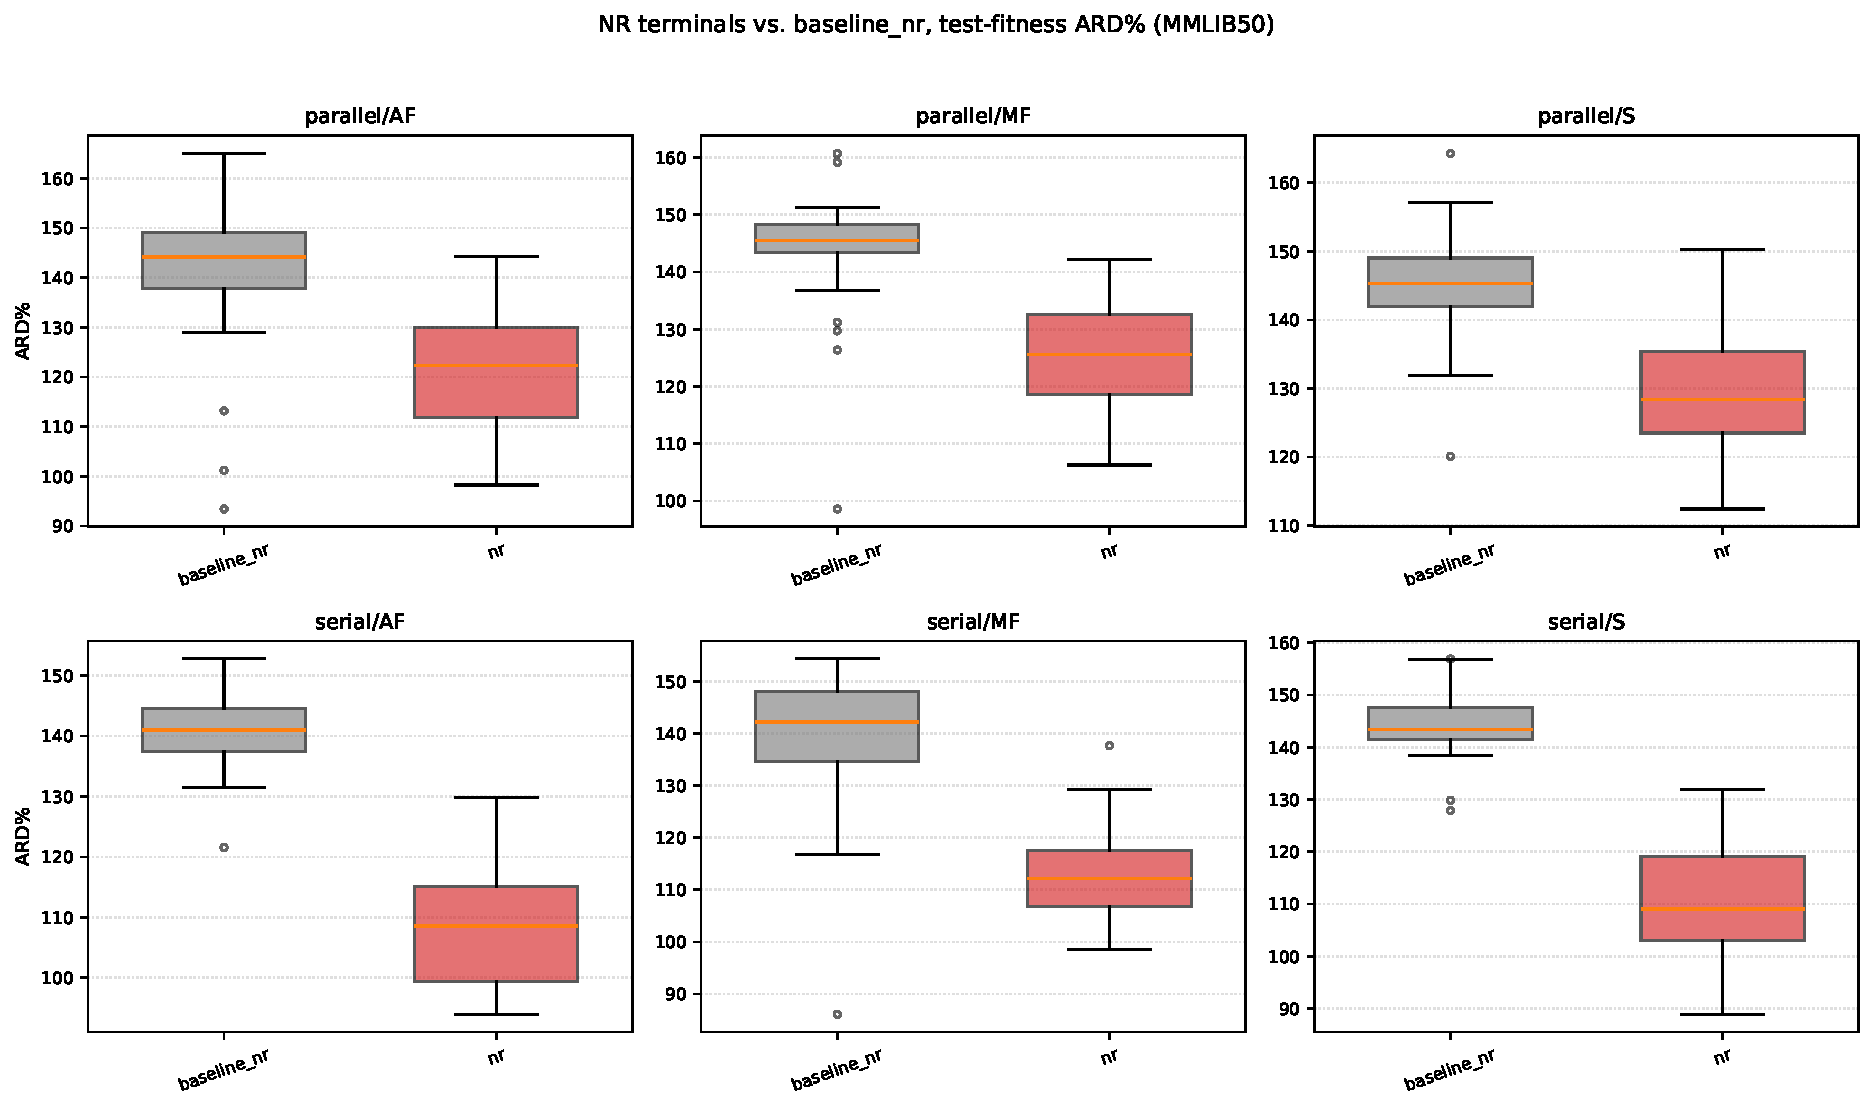
\includegraphics[width=0.95\textwidth]{img/generated/nr_boxplot_mmlib50.pdf}
  \caption{Distribution of test-fitness ARD\%, NR terminals vs.\
  \texttt{baseline\_nr}, MMLIB50 NR-preserving instances, one panel per
  (SGS, strategy) cell, 30 seeds per box. Note the much larger ARD\% scale
  than Figures~\ref{fig:lexicase-boxplot}/\ref{fig:localsearch-boxplot},
  a consequence of the looser CPM lower bound on NR-preserving instances
  (Section~\ref{subsec:threats-construct}), not of the algorithms
  themselves.}
  \label{fig:nr-boxplot}
\end{figure}

\begin{figure}[htbp]
  \centering
  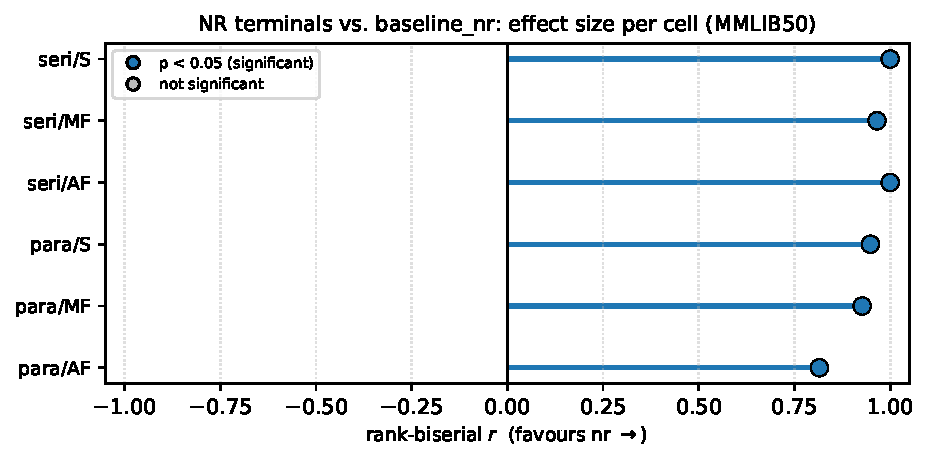
\includegraphics[width=0.85\textwidth]{img/generated/nr_effectsize_mmlib50.pdf}
  \caption[Effect-size summary, NR terminals vs.\ baseline\_nr]{Effect-size
  summary, NR terminals vs.\ \texttt{baseline\_nr}, MMLIB50: matched
  rank-biserial correlation $r$ per (SGS, strategy) cell (positive favours
  NR terminals), filled markers denote $p<0.05$; every cell is significant
  and favourable, see Figure~\ref{fig:lexicase-cd}'s caption for why a
  per-cell effect-size plot, not a Nemenyi CD diagram, is used for this
  two-condition comparison.}
  \label{fig:nr-cd}
\end{figure}

\begin{table}[htbp]
  \centering
  \small
  \shrinktofit{%
  \caption[NR terminals vs.\ baseline on MMLIB100]{Mean ARD\% (\%),
  \texttt{baseline\_nr} vs.\ NR terminals, MMLIB100 (NR-preserving
  instances, scalability validation), $n=30$ seeds per cell.
  \changedC{Each mean is taken only over the instances a rule scheduled
  feasibly; infeasible instances receive no penalty value and are instead
  reported separately as the feasibility rate in
  Table~\ref{tab:nr-descriptive-stats-mmlib100}. Because the two
  conditions differ in feasibility, their means cover different instance
  subsets, so the two tables must be read together.}}
  \label{tab:nr-vs-baseline-mmlib100}
  \begin{tabular}{llrrrr}
    \toprule
    \textbf{SGS} & \textbf{Strategy} & \textbf{\texttt{baseline\_nr} (test)} & \textbf{NR terminals (test)} & \textbf{\texttt{baseline\_nr} (train)} & \textbf{NR terminals (train)} \\
    \midrule
    Parallel & AF & 114.37 & 113.77\,\ArrBetter & 107.46 & 108.28\,\ArrWorse \\
    Parallel & MF & 113.68 & 114.34\,\ArrWorse & 106.25 & 108.46\,\ArrWorse \\
    Parallel & S  & 124.88 & 110.56\,\ArrBetter & 115.22 & 105.15\,\ArrBetter \\
    Serial   & AF & 118.46 &  90.07\,\ArrBetter & 110.18 &  83.68\,\ArrBetter \\
    Serial   & MF & 116.98 &  89.85\,\ArrBetter & 108.51 &  83.45\,\ArrBetter \\
    Serial   & S  & 124.49 &  83.16\,\ArrBetter & 116.33 &  78.59\,\ArrBetter \\
    \bottomrule
  \end{tabular}%
  }
\end{table}

\begin{table}[htbp]
  \centering
  \small
  \shrinktofit{%
  \caption[Descriptive statistics: NR terminals vs.\ baseline, MMLIB100]{\changedC{Standard
  deviation and feasibility rate accompanying
  Table~\ref{tab:nr-vs-baseline-mmlib100}, MMLIB100. The feasibility gain
  replicates at the larger scale in every cell, though from a higher
  baseline and by a smaller margin than on MMLIB50: held-out test
  feasibility rises from roughly 75--88\% under \texttt{baseline\_nr} to
  roughly 87--93\% under NR terminals.}}
  \label{tab:nr-descriptive-stats-mmlib100}
  \begin{tabular}{lllrrrr}
    \toprule
    \textbf{SGS} & \textbf{Strategy} & \textbf{Split} & \textbf{\texttt{baseline\_nr} std} & \textbf{NR std} & \textbf{\texttt{baseline\_nr} feas.} & \textbf{NR feas.} \\
    \midrule
    Parallel & AF & Train &  8.66 &  6.43 & 0.91 & 0.99 \\
    Parallel & AF & Test  & 11.42 &  8.17 & 0.75 & 0.89 \\
    Parallel & MF & Train & 11.76 &  7.82 & 0.91 & 0.98 \\
    Parallel & MF & Test  & 14.32 &  8.27 & 0.75 & 0.87 \\
    Parallel & S  & Train & 11.52 &  7.10 & 0.91 & 1.00 \\
    Parallel & S  & Test  & 14.97 &  9.77 & 0.78 & 0.88 \\
    Serial   & AF & Train &  9.16 &  4.52 & 0.99 & 1.00 \\
    Serial   & AF & Test  & 11.43 &  4.64 & 0.83 & 0.93 \\
    Serial   & MF & Train &  8.12 &  4.02 & 1.00 & 1.00 \\
    Serial   & MF & Test  &  9.98 &  5.04 & 0.85 & 0.90 \\
    Serial   & S  & Train &  8.21 & 10.31 & 0.98 & 1.00 \\
    Serial   & S  & Test  & 11.00 & 12.89 & 0.88 & 0.91 \\
    \bottomrule
  \end{tabular}%
  }
\end{table}

\begin{table}[htbp]
  \centering
  \small
  \shrinktofit{%
  \caption[Statistical significance: NR terminals vs.\ baseline, MMLIB100]{Two-sided
  paired Wilcoxon signed-rank test and matched rank-biserial effect size
  $r$, NR terminals vs.\ \texttt{baseline\_nr}, MMLIB100.}
  \label{tab:nr-significance-mmlib100}
  \begin{tabular}{lllrrl}
    \toprule
    \textbf{SGS} & \textbf{Strategy} & \textbf{Split} & \textbf{$p$} & \textbf{$r$} & \textbf{Verdict} \\
    \midrule
    Parallel & AF & Train & 0.6408 & $-0.101$ & Not significant \\
    Parallel & AF & Test  & 0.7151 & $+0.080$ & Not significant \\
    Parallel & MF & Train & 0.4400 & $-0.166$ & Not significant \\
    Parallel & MF & Test  & 0.7766 & $-0.062$ & Not significant \\
    Parallel & S  & Train & 0.0005 & $+0.695$ & Significant, favours NR terminals \\
    Parallel & S  & Test  & 0.0002 & $+0.742$ & Significant, favours NR terminals \\
    Serial   & AF & Train & $<0.0001$ & $+1.000$ & Significant, favours NR terminals \\
    Serial   & AF & Test  & $<0.0001$ & $+1.000$ & Significant, favours NR terminals \\
    Serial   & MF & Train & $<0.0001$ & $+1.000$ & Significant, favours NR terminals \\
    Serial   & MF & Test  & $<0.0001$ & $+0.996$ & Significant, favours NR terminals \\
    Serial   & S  & Train & $<0.0001$ & $+1.000$ & Significant, favours NR terminals \\
    Serial   & S  & Test  & $<0.0001$ & $+1.000$ & Significant, favours NR terminals \\
    \bottomrule
  \end{tabular}%
  }
\end{table}

\begin{figure}[htbp]
  \centering
  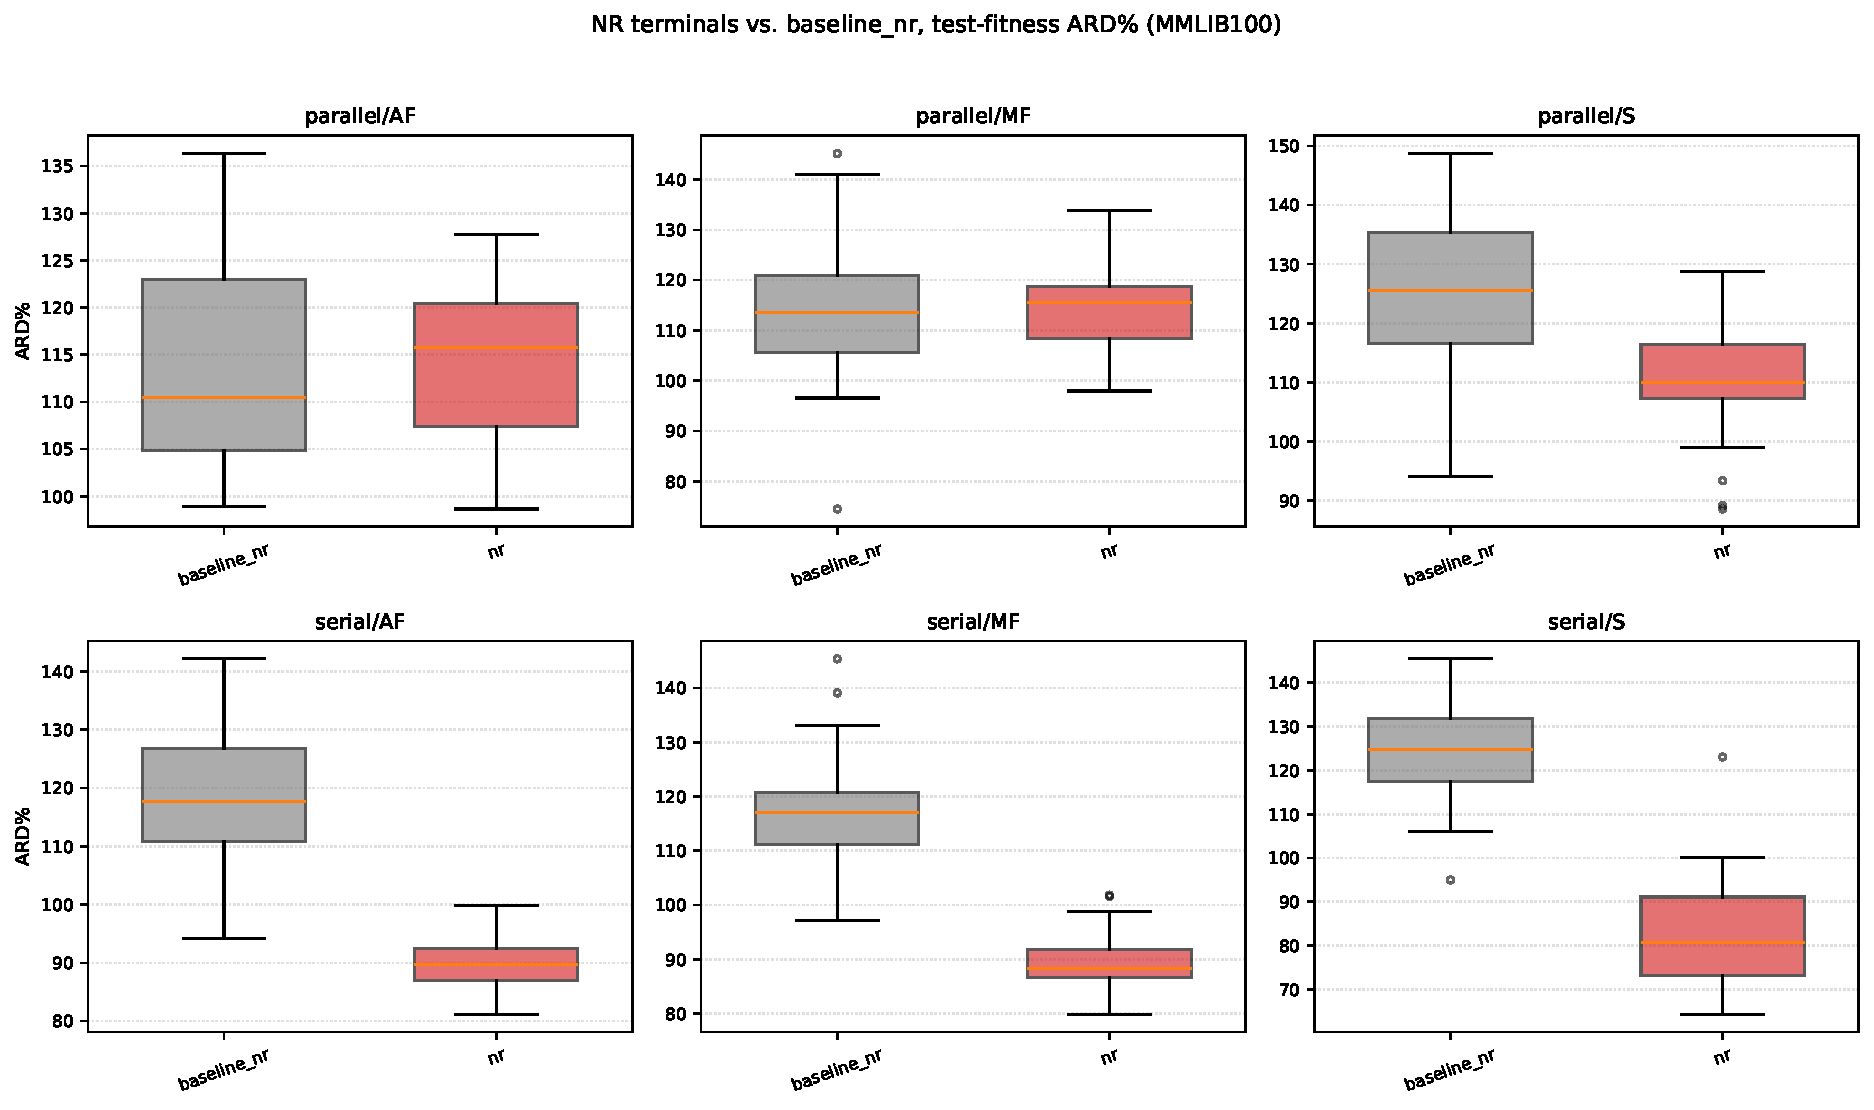
\includegraphics[width=0.95\textwidth]{img/generated/nr_boxplot_mmlib100.pdf}
  \caption{Distribution of test-fitness ARD\%, NR terminals vs.\
  \texttt{baseline\_nr}, MMLIB100, same layout as Figure~\ref{fig:nr-boxplot}.
  Note the visibly overlapping boxes in the two parallel/AF and parallel/MF
  panels, contrasting with the clear separation in the other four.}
  \label{fig:nr-boxplot-mmlib100}
\end{figure}

\begin{figure}[htbp]
  \centering
  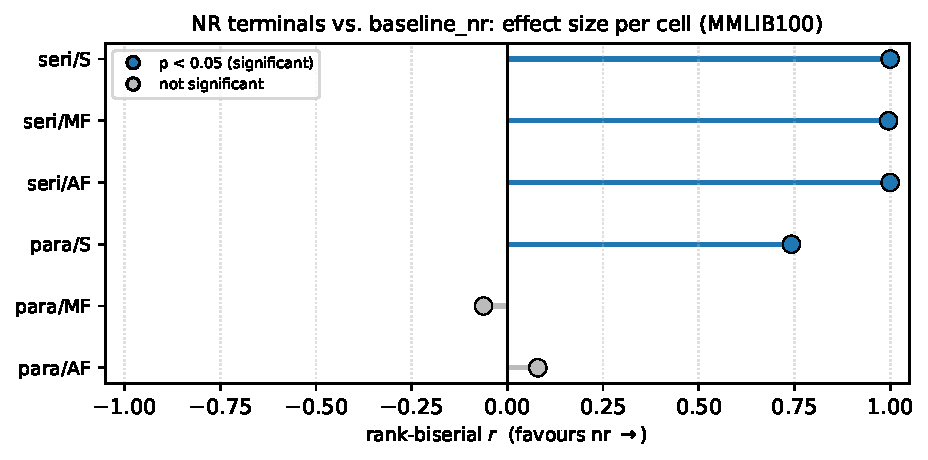
\includegraphics[width=0.85\textwidth]{img/generated/nr_effectsize_mmlib100.pdf}
  \caption[Effect-size summary, NR terminals vs.\ baseline\_nr, MMLIB100]{Effect-size
  summary, NR terminals vs.\ \texttt{baseline\_nr}, MMLIB100: four cells
  remain strongly favourable and significant, while parallel/AF and
  parallel/MF collapse toward zero, the visual counterpart of
  Table~\ref{tab:nr-significance-mmlib100}.}
  \label{fig:nr-cd-mmlib100}
\end{figure}

On \textbf{MMLIB50}, this is, by a wide margin, the most robust result in
this chapter. Every one of the twelve train/test comparisons across all six
(SGS, strategy) cells reaches significance at $p<0.0001$ with a large
effect size ($r \geq 0.815$), and, unlike either selection or local search,
the effect is stable in both sign and magnitude across every decoding
scheme and every GP decision strategy: there is no SGS-dependent reversal
here of the kind seen in Sections~\ref{subsec:lexicase-eval}
and~\ref{subsec:localsearch-eval}. \changedC{The mechanism behind this is
straightforward:}
without any NR signal, the baseline can only avoid exhausting the project's
non-renewable budget by chance, and Table~\ref{tab:nr-descriptive-stats}
shows this directly in the feasibility rate, not just the mean. Held-out
test feasibility rises from roughly 68--70\% under \texttt{baseline\_nr} to
roughly 82--86\% under NR terminals in every single cell, meaning the
improvement is not solely a matter of NR terminals producing modestly
better schedules on the instances both conditions could already solve; it
is also solving a meaningfully larger share of instances that the baseline
could not solve at all. \changedB{One qualification to this feasibility
gain is established later: re-evaluated on the complete 108-class test
set, it proves largely confined to the instance classes seen during
training, while the schedule-quality advantage carries over in full
(Section~\ref{subsec:full108}).}

\textbf{Scalability validation.} Table~\ref{tab:nr-significance-mmlib100}
qualifies \changed{these results} in a specific and informative way rather than
simply confirming them. Four of the six MMLIB100 cells, both serial/AF,
serial/MF, serial/S and, notably, parallel/S, replicate MMLIB50's result
almost exactly, large, significant effects on both train and test fitness
($r=0.695$--$1.000$). The remaining two cells, parallel/AF and
parallel/MF, do not: at MMLIB100 scale neither the training-fitness nor the
test-fitness advantage reaches significance ($p=0.44$--$0.78$, $|r|\leq
0.17$), a marked change from MMLIB50's own parallel/AF and parallel/MF rows,
which were both significant there ($r=0.815$--$0.987$). This is a genuine,
specific scale-dependence, not a uniform weakening: NR terminals' benefit
is confirmed as robust to instance size under serial SGS (all three
strategies) and under parallel/simultaneous, but does not clearly survive
scaling from MMLIB50 to MMLIB100 under parallel/activity-first or
parallel/mode-first. \changedC{The feasibility side of the result is more
uniform: Table~\ref{tab:nr-descriptive-stats-mmlib100} shows NR terminals
raising the held-out feasibility rate in all six cells at MMLIB100,
including the two whose fitness advantage vanishes, so what fails to
replicate in parallel/AF and parallel/MF is the schedule-quality gain,
not the ability to find feasible schedules. Read together with the
feasible-only convention stated above, those two cells' near-equal mean
ARD\% is if anything conservative: the NR condition achieves it while
feasibly scheduling a larger, and therefore presumably harder, share of
the test instances.}

The cells that fail share a specific structural property the cells that
succeed do not, which points to a concrete mechanism rather than a vague
``more complexity'' explanation. Activity-first and mode-first both split
the decision into two independently evolved trees (Section~\ref{subsec:individual-representation}):
the activity tree sees \texttt{NR\_STOCK\_RATIO}/\texttt{NR\_BUDGET\_PRESSURE},
the mode tree sees \texttt{NR\_MODE\_DEMAND\_RATIO}, and the two trees can
only coordinate an NR-aware trade-off implicitly, through the shared
fitness signal, never within a single expression. Simultaneous mode uses
one integrated tree that scores each (activity, mode) pair jointly, so it
can encode a rule like ``favour this activity only if some mode of it
keeps NR demand low'' directly, with both signals visible to the same
expression at the same time. Parallel SGS is precisely the decoding scheme
that stresses the split-tree architecture's coordination gap: unlike serial
SGS, which commits one activity/mode pair at a time and updates the
remaining NR budget immediately afterwards, parallel SGS advances a single
global clock and can commit \emph{several} activities' mode choices within
the same time step, all drawing against the same NR budget before it is
next updated. Coordinating that many simultaneous, mutually competing
NR-relevant choices correctly is exactly the kind of joint reasoning an
integrated tree can express directly and two decoupled trees can only
approximate through indirect selection pressure. MMLIB100's larger
instances make this \changed{harder}:
more activities per instance means more candidate activities are typically
eligible, and hence more simultaneous mode decisions are competing for the
same shrinking NR budget within a single parallel-SGS time step, than on
MMLIB50's smaller instances. Simultaneous mode is insulated from this
because it never had to solve the coordination problem in the first place;
serial SGS is insulated because it never presents the simultaneous
contention that makes the coordination problem hard. Activity-first and
mode-first under parallel SGS are the one combination exposed to both the
coordination gap and \changed{the scale at which it becomes decisive. This
account is consistent with} Section~\ref{subsec:localsearch-eval}'s
observation that parallel SGS's simultaneous commits leave more exploitable
structure in the resulting schedule than serial SGS's one-at-a-time
construction: the same architectural difference between the two decoding
schemes that gives local search more to work with under parallel SGS is
what gives a split-tree NR rule more simultaneous contention to fail to
coordinate. Directly testing this account, for instance by comparing how
often activity-first/mode-first's two trees make internally consistent
NR-aware choices within the same parallel-SGS time step versus how often
they contradict each other, is left as future work
(Section~\ref{sec:future-work}). Even with this qualification, NR terminals
remain this thesis's strongest and most broadly replicated result: unlike
lexicase (which weakens further at MMLIB100) or local search (whose one
significant MMLIB50 win disappears entirely), four of NR terminals' six
cells replicate cleanly, and none reverses direction.

Two further caveats qualify, without undermining, this result. First,
because \texttt{nr} necessarily runs on a different instance set
(NR-preserving) than \texttt{baseline}, \texttt{lexicase}, and
\texttt{local\_search} above, this comparison cannot be \changedD{included in} the
same six-cell, four-condition ranking used in
Section~\ref{subsec:final-comparison}\changed{; it is therefore reported
here as its own, self-contained result}. Second,
generalisation to instances harder than MMLIB100, in particular MMLIB+'s
tighter NR budgets, is not established by this section; a separate,
smaller-scale, instance-matched study (referenced in the repository's own
experiment log) found the same direction of effect on MMLIB+ but with
markedly higher test infeasibility for both conditions, a question
Section~\ref{sec:future-work} returns to.

\changedB{Beyond the aggregate statistics, it is worth looking at what the
NR-aware GPHH actually evolves. Figure~\ref{fig:nr-evolved-tree} shows a
compact evolved rule pair from the serial/activity-first cell, chosen as the
smallest run (by total node count) that still recruits the non-renewable
terminals in both trees, so the mechanism is legible without the visual
clutter of a larger individual. Both trees reference the new terminals
without any prompting: the activity tree gates its priority on
\texttt{NR\_STOCK\_RATIO}, so activities are ordered partly by how much of
the non-renewable budget remains, while the mode tree is dominated by
\texttt{NR\_MODE\_DEMAND\_RATIO}\changedC{, penalising modes whose
non-renewable demand is high relative to what is left. The evolved
individual references that terminal four times, but two of the four form a
subtree dividing it by itself, which under protected division is the
constant $1$, a typical piece of functionally neutral code that GP trees
accumulate;
Figure~\ref{fig:nr-evolved-tree} omits one of that subtree's two identical
operands for legibility, so the terminal is drawn three times there. The
two \changedD{remaining} references each divide \texttt{NR\_MODE\_DEMAND\_RATIO} by
the resource-count terminal \texttt{RR}. This is direct evidence that the
improvement reported above comes from the rule actually using the new
information rather than from some incidental side effect of enlarging the
terminal set:} given visibility into the non-renewable state,
evolution places those terminals at \changedD{important} positions in the rule
rather than leaving them as unused vocabulary.}
\changedC{Nor is this recruitment specific to the displayed pair: across
all of the \texttt{nr} condition's champions (the champion-wide analysis
of Section~\ref{subsec:localsearch-eval}),
\texttt{NR\_MODE\_DEMAND\_RATIO} is recruited by every single mode and
integrated tree ($100\%$ under both SGS), \texttt{NR\_STOCK\_RATIO}
appears in $81\%$ of the parallel activity trees, and
\texttt{NR\_BUDGET\_PRESSURE} in about three quarters of the serial
ones, so the new terminals are, population-wide, among the most
recruited vocabulary the rules have.}

\begin{figure}[htbp]
  \centering
  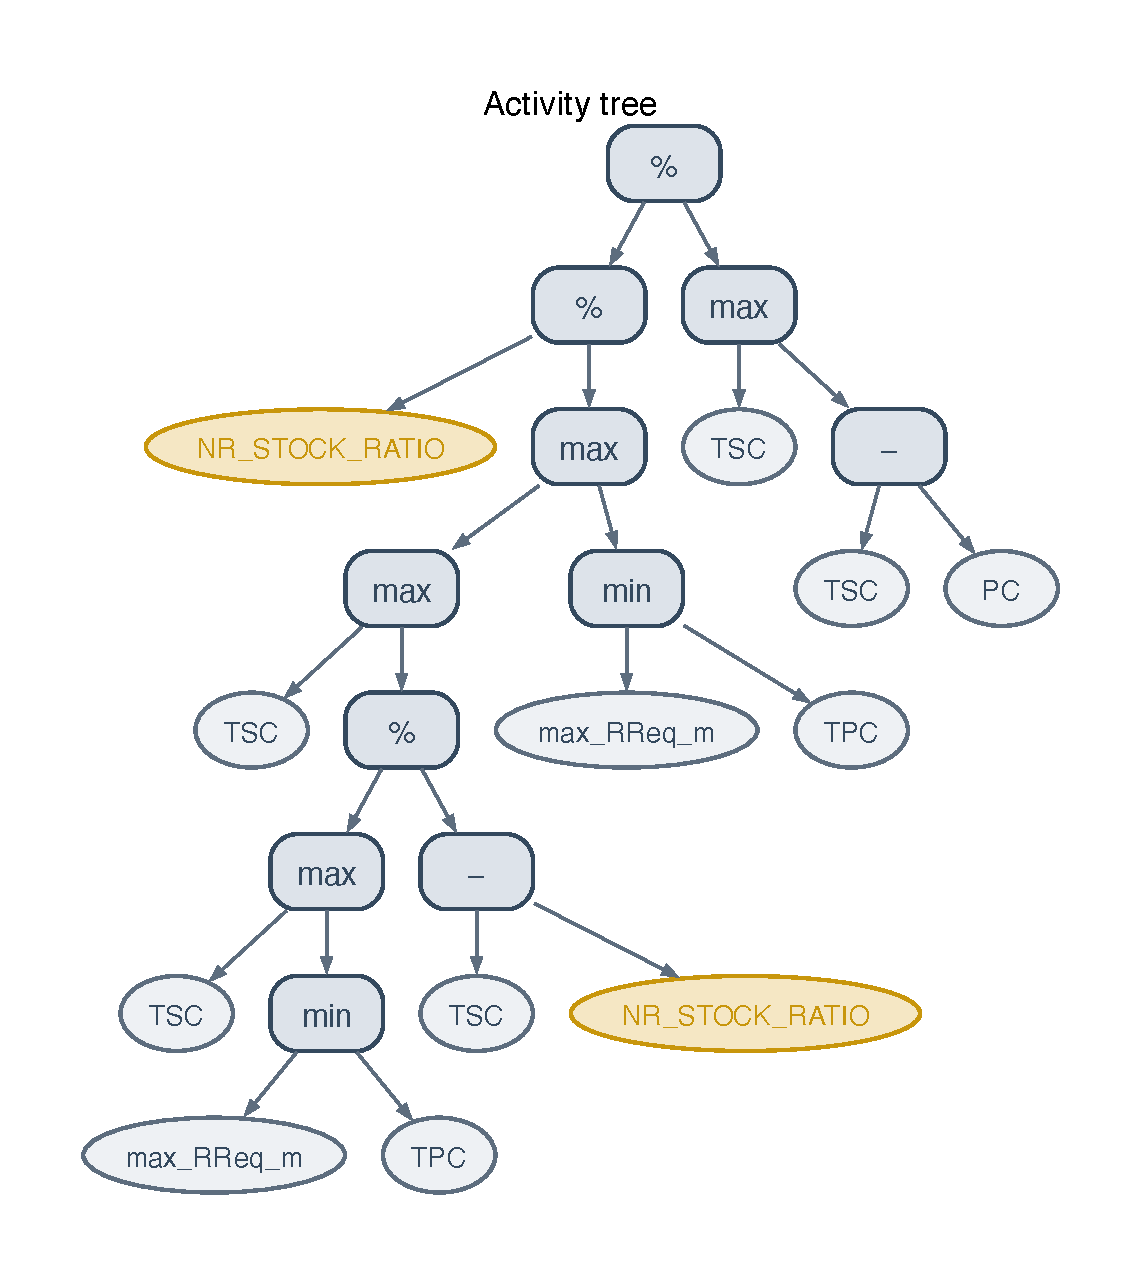
\includegraphics[width=0.62\textwidth]{img/generated/gp_tree_evolved_activity.pdf}\\[1.5ex]
  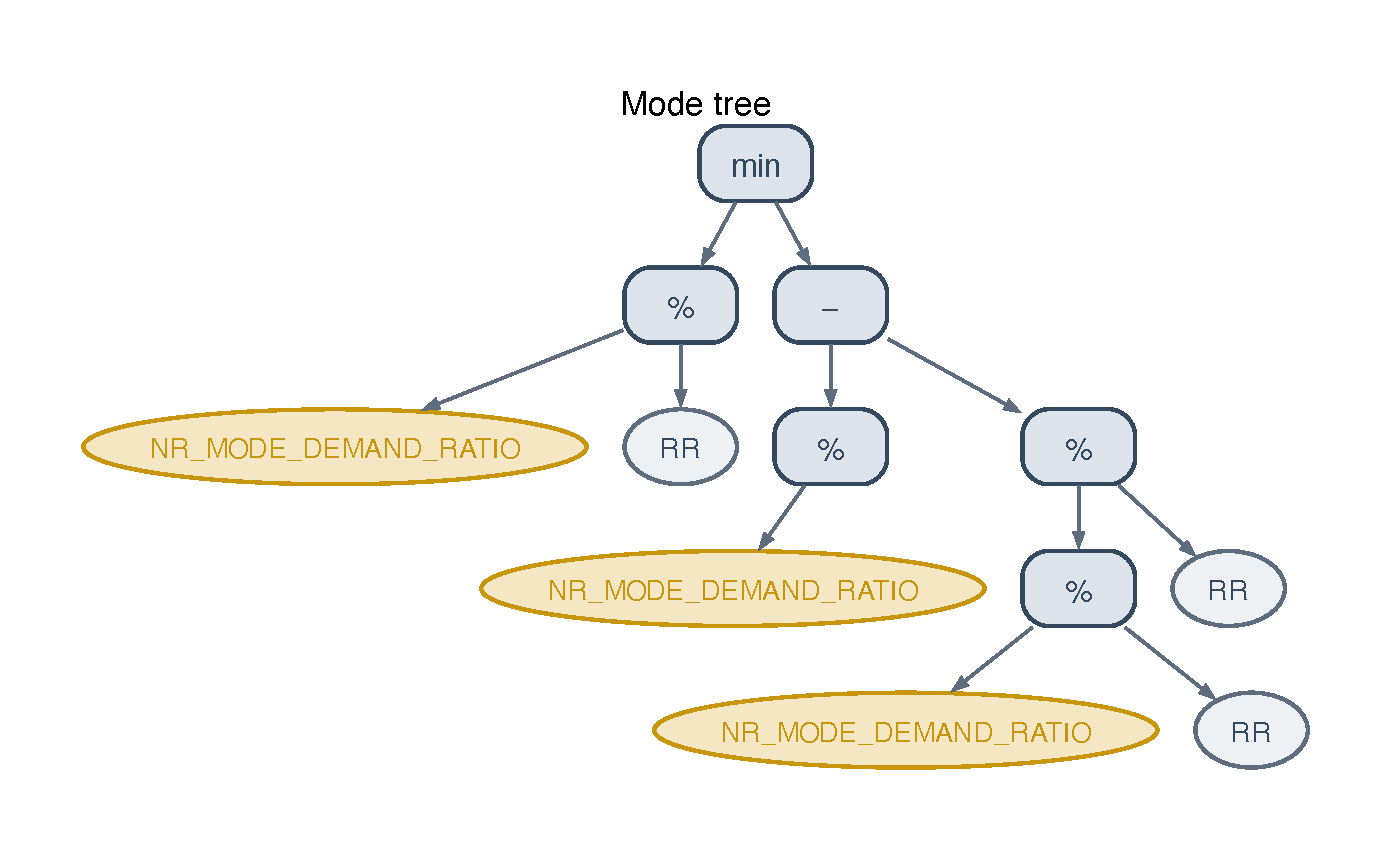
\includegraphics[width=0.98\textwidth]{img/generated/gp_tree_evolved_mode.pdf}
  \caption[Evolved NR-aware rule pair]{\changedB{A compact evolved NR-aware
  rule pair (serial/activity-first, MMLIB50), selected as the smallest
  individual that recruits the non-renewable terminals in both trees.
  Top: the activity tree, which selects the next activity to schedule.
  Bottom: the mode tree, which selects its execution mode. Operator nodes are
  blue; ordinary terminals are grey; the non-renewable terminals contributed
  by this work (\texttt{NR\_STOCK\_RATIO},
  \texttt{NR\_MODE\_DEMAND\_RATIO}) are highlighted in gold. The GP function
  set is $\{+, -, \times, \%, \min, \max\}$, where $\%$ denotes protected
  division.}}
  \label{fig:nr-evolved-tree}
\end{figure}

\section{Benchmark evaluation and baseline comparison}
\label{sec:benchmark-comparison}

Sections~\ref{subsec:lexicase-eval} through~\ref{subsec:nr-eval} each
compared one candidate modification against its own matched baseline in
isolation, which answers whether that specific modification helps but not
how the modifications compare against one another or which, if any, would
be the single configuration worth recommending. This section closes that
gap: it ranks baseline, lexicase, local search, and hybrid jointly on the
same six-cell grid, reports NR terminals' result alongside for qualitative
reference, and summarises what the comprehensive stage as a whole,
MMLIB50's complete grid together with MMLIB100's scalability check,
supports as this thesis's final, evidence-based verdict.

\subsection{Final comparison and summary}
\label{subsec:final-comparison}

\changed{The four jointly ranked conditions are baseline, lexicase, local
search, and hybrid (lexicase selection and local search applied together),
compared with the average-rank and Friedman methodology of
Section~\ref{subsec:statistical-methodology}.}

\begin{table}[htbp]
  \centering
  \small
  \shrinktofit{%
  \caption[Method rankings]{Average rank (1 = best, 4 = worst) across the
  six (SGS, strategy) cells, MMLIB50, test and train fitness. The test-rank
  Friedman test is significant ($\chi^2 = 10.20$, $p = 0.0169$, 6 blocks, 4
  conditions); the train-rank Friedman test is not ($\chi^2 = 0.20$,
  $p = 0.978$).}
  \label{tab:method-rankings}
  \begin{tabular}{lrrrr}
    \toprule
    \textbf{Condition} & \textbf{Avg.\ rank (test)} & \textbf{Avg.\ rank (train)} \\
    \midrule
    Local search & 1.50 & 2.67 \\
    Baseline     & 2.33 & 2.50 \\
    Lexicase     & 2.33 & 2.50 \\
    Hybrid       & 3.83 & 2.33 \\
    \bottomrule
  \end{tabular}%
  }
\end{table}

\begin{table}[htbp]
  \centering
  \small
  \shrinktofit{%
  \caption[Final comparison on MMLIB50]{Final side-by-side comparison of
  all four jointly ranked conditions, mean test-fitness ARD\% (\%),
  MMLIB50, the same six rows underlying Table~\ref{tab:method-rankings}'s
  ranks. *NR terminals' own result is appended for qualitative reference
  only: it runs on NR-preserving instances against \texttt{baseline\_nr},
  not the renewable-only-converted instances the other four columns share,
  so it is \emph{not} on the same ARD\% scale and must not be compared
  numerically against the other columns (Section~\ref{subsec:nr-eval}).}
  \label{tab:final-comparison-mmlib50}
  \begin{tabular}{llrrrrr}
    \toprule
    \textbf{SGS} & \textbf{Strategy} & \textbf{Baseline} & \textbf{Lexicase} & \textbf{Local search} & \textbf{Hybrid} & \textbf{NR terminals*} \\
    \midrule
    Parallel & AF & 35.77 & 34.36\,\ArrBetter & 33.64\,\ArrBetter & 34.51\,\ArrBetter & 121.74 \\
    Parallel & MF & 35.78 & 35.50\,\ArrBetter & 35.57\,\ArrBetter & 36.08\,\ArrWorse & 124.85 \\
    Parallel & S  & 30.43 & 30.08\,\ArrBetter & 29.79\,\ArrBetter & 30.72\,\ArrWorse & 129.27 \\
    Serial   & AF & 17.81 & 18.33\,\ArrWorse & 18.24\,\ArrWorse & 18.56\,\ArrWorse & 109.23 \\
    Serial   & MF & 17.89 & 18.52\,\ArrWorse & 18.37\,\ArrWorse & 19.08\,\ArrWorse & 113.54 \\
    Serial   & S  & 18.08 & 18.41\,\ArrWorse & 17.77\,\ArrBetter & 18.43\,\ArrWorse & 110.37 \\
    \bottomrule
  \end{tabular}%
  }
\end{table}

\begin{figure}[htbp]
  \centering
  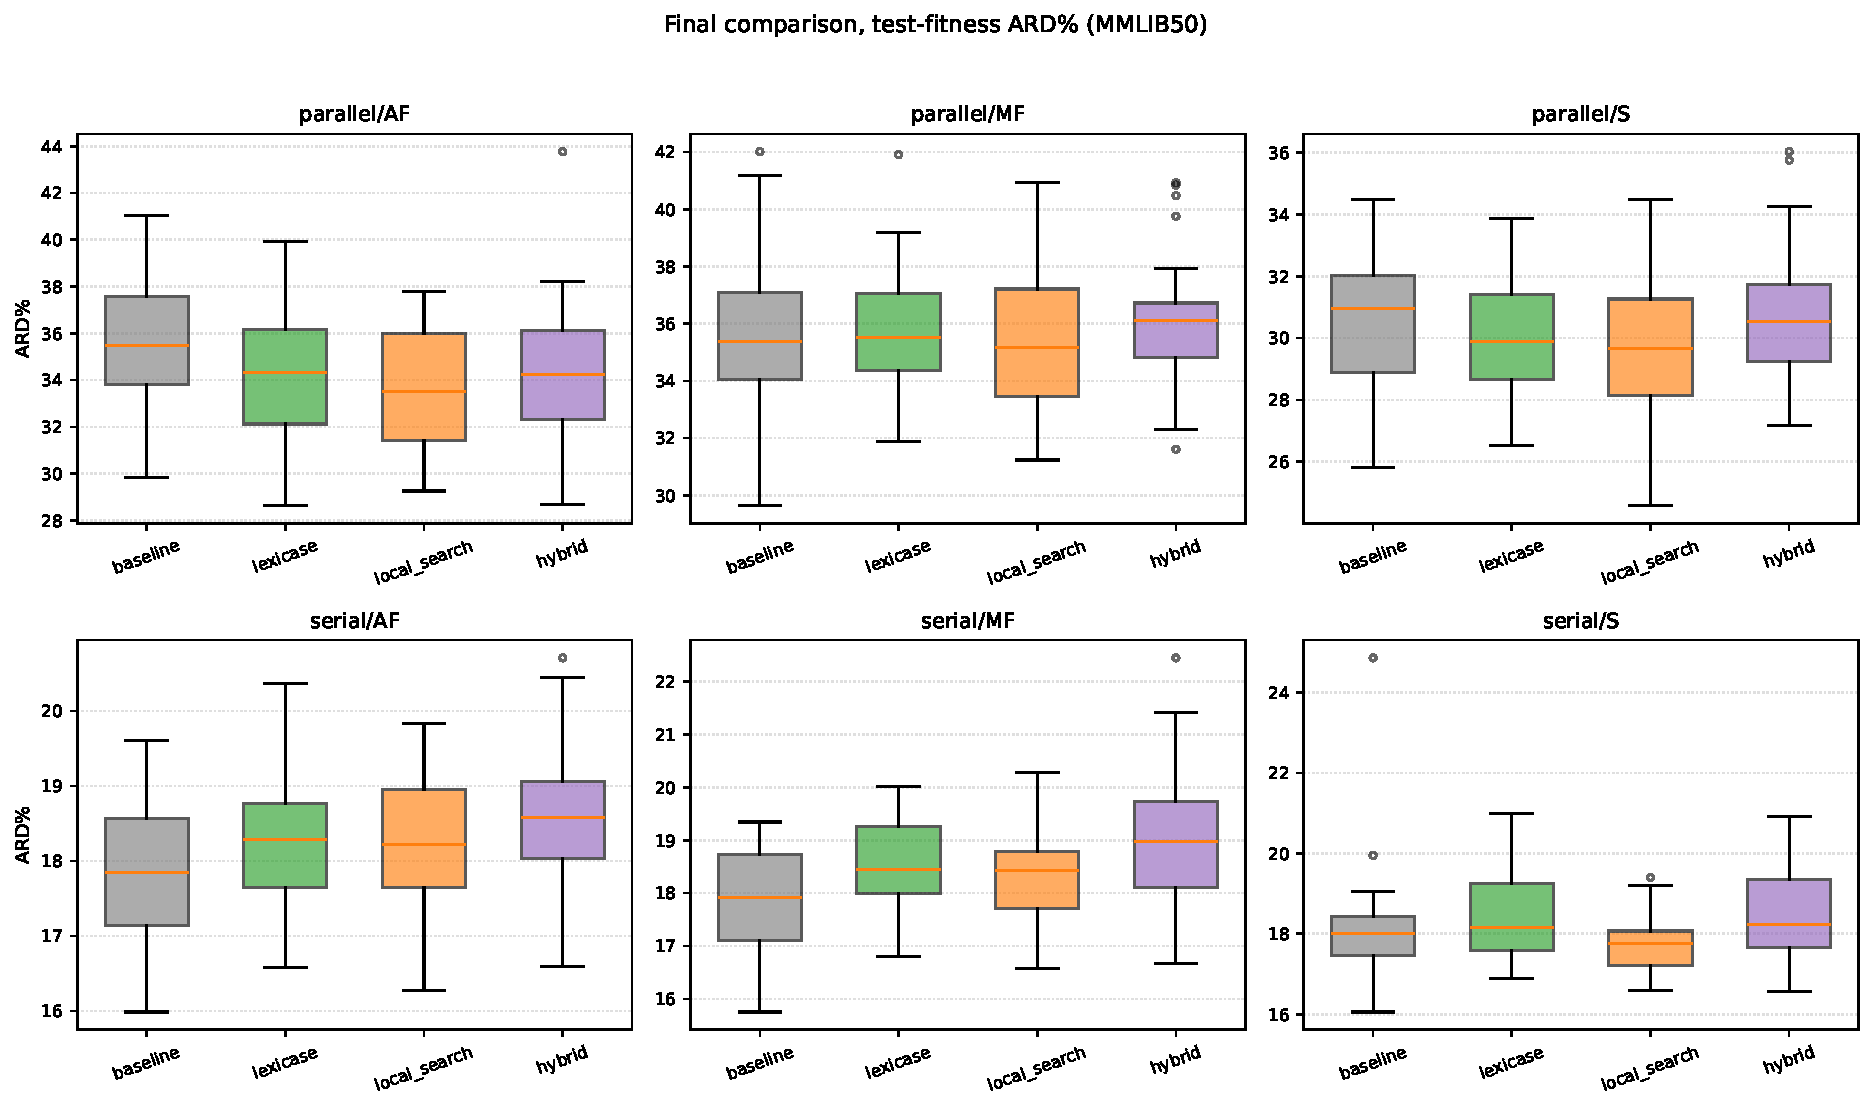
\includegraphics[width=0.95\textwidth]{img/generated/final_comparison_boxplot_mmlib50.pdf}
  \caption{Final comparison boxplot, all four jointly ranked conditions,
  MMLIB50, one panel per (SGS, strategy) cell.}
  \label{fig:final-comparison-boxplot}
\end{figure}

\begin{figure}[htbp]
  \centering
  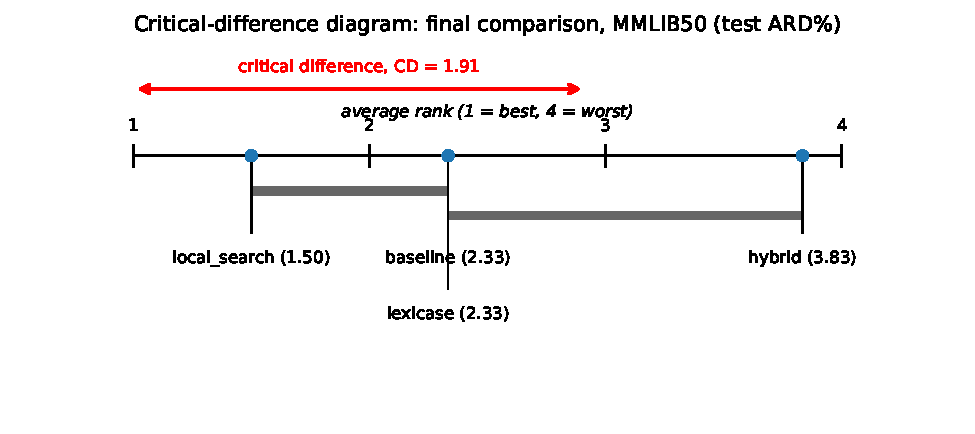
\includegraphics[width=0.85\textwidth]{img/generated/final_comparison_cd_mmlib50.pdf}
  \caption[Critical-difference diagram, final comparison, MMLIB50]{Critical-difference
  diagram, final comparison, MMLIB50 (test ARD\%). The Friedman test is
  significant ($p=0.0169$), so this diagram is meaningful: local search
  separates from hybrid by more than the critical difference (CD $=1.91$),
  while baseline and lexicase, tied at average rank 2.33, sit between them
  and are not statistically distinguishable from either.}
  \label{fig:final-comparison-cd}
\end{figure}

Figure~\ref{fig:final-comparison-cd} packs several pieces of information
into one plot, so it is worth reading it element by element. The
horizontal axis is average rank across the six (SGS, strategy) cells,
running from 1 (best, i.e.\ lowest mean ARD\%) to 4 (worst); each
condition's dot marks its own average rank from
Table~\ref{tab:method-rankings} (local search 1.50, baseline and lexicase
tied at 2.33, hybrid 3.83). The red double-headed arrow at the top is not a
comparison between two specific conditions: it is a ruler, showing how long
one critical difference (CD $=1.91$ rank units, computed from the Nemenyi
formula for $k=4$ conditions and $N=6$ blocks/cells) is on this axis, so
the reader can visually judge distances between dots against it. The thick
grey bars beneath the axis are the actual pairwise verdicts: a bar spanning
two or more dots means those conditions' average ranks are \emph{closer
together than one CD}, i.e.\ not distinguishable from chance at this
sample size; conditions with \emph{no} bar connecting them (here, local
search and hybrid, $3.83-1.50=2.33 > \mathrm{CD}$) are the pairs the
diagram identifies as genuinely different. Reading the two bars together:
local search's rank is close enough to baseline/lexicase's to share a bar
with them, and baseline/lexicase's rank is in turn close enough to
hybrid's to share a second, separate bar with it, but local search and
hybrid themselves, at the two ends, are far enough apart that no single bar
spans both, which is exactly what \changedC{``local search significantly
outranks hybrid, with baseline and lexicase in between and not clearly
separable from either neighbour''} looks like in this convention.

\begin{table}[htbp]
  \centering
  \small
  \caption[Method rankings, MMLIB100]{Average rank (1 = best, 4 = worst)
  across the six (SGS, strategy) cells, MMLIB100, test and train fitness.
  Neither Friedman test is significant (test: $\chi^2 = 1.40$, $p = 0.706$;
  train: $\chi^2 = 4.20$, $p = 0.241$; 6 blocks, 4 conditions).}
  \label{tab:method-rankings-mmlib100}
  \begin{tabular}{lrr}
    \toprule
    \textbf{Condition} & \textbf{Avg.\ rank (test)} & \textbf{Avg.\ rank (train)} \\
    \midrule
    Baseline     & 2.00 & 2.50 \\
    Lexicase     & 2.50 & 1.67 \\
    Hybrid       & 2.67 & 2.67 \\
    Local search & 2.83 & 3.17 \\
    \bottomrule
  \end{tabular}
\end{table}

\begin{figure}[htbp]
  \centering
  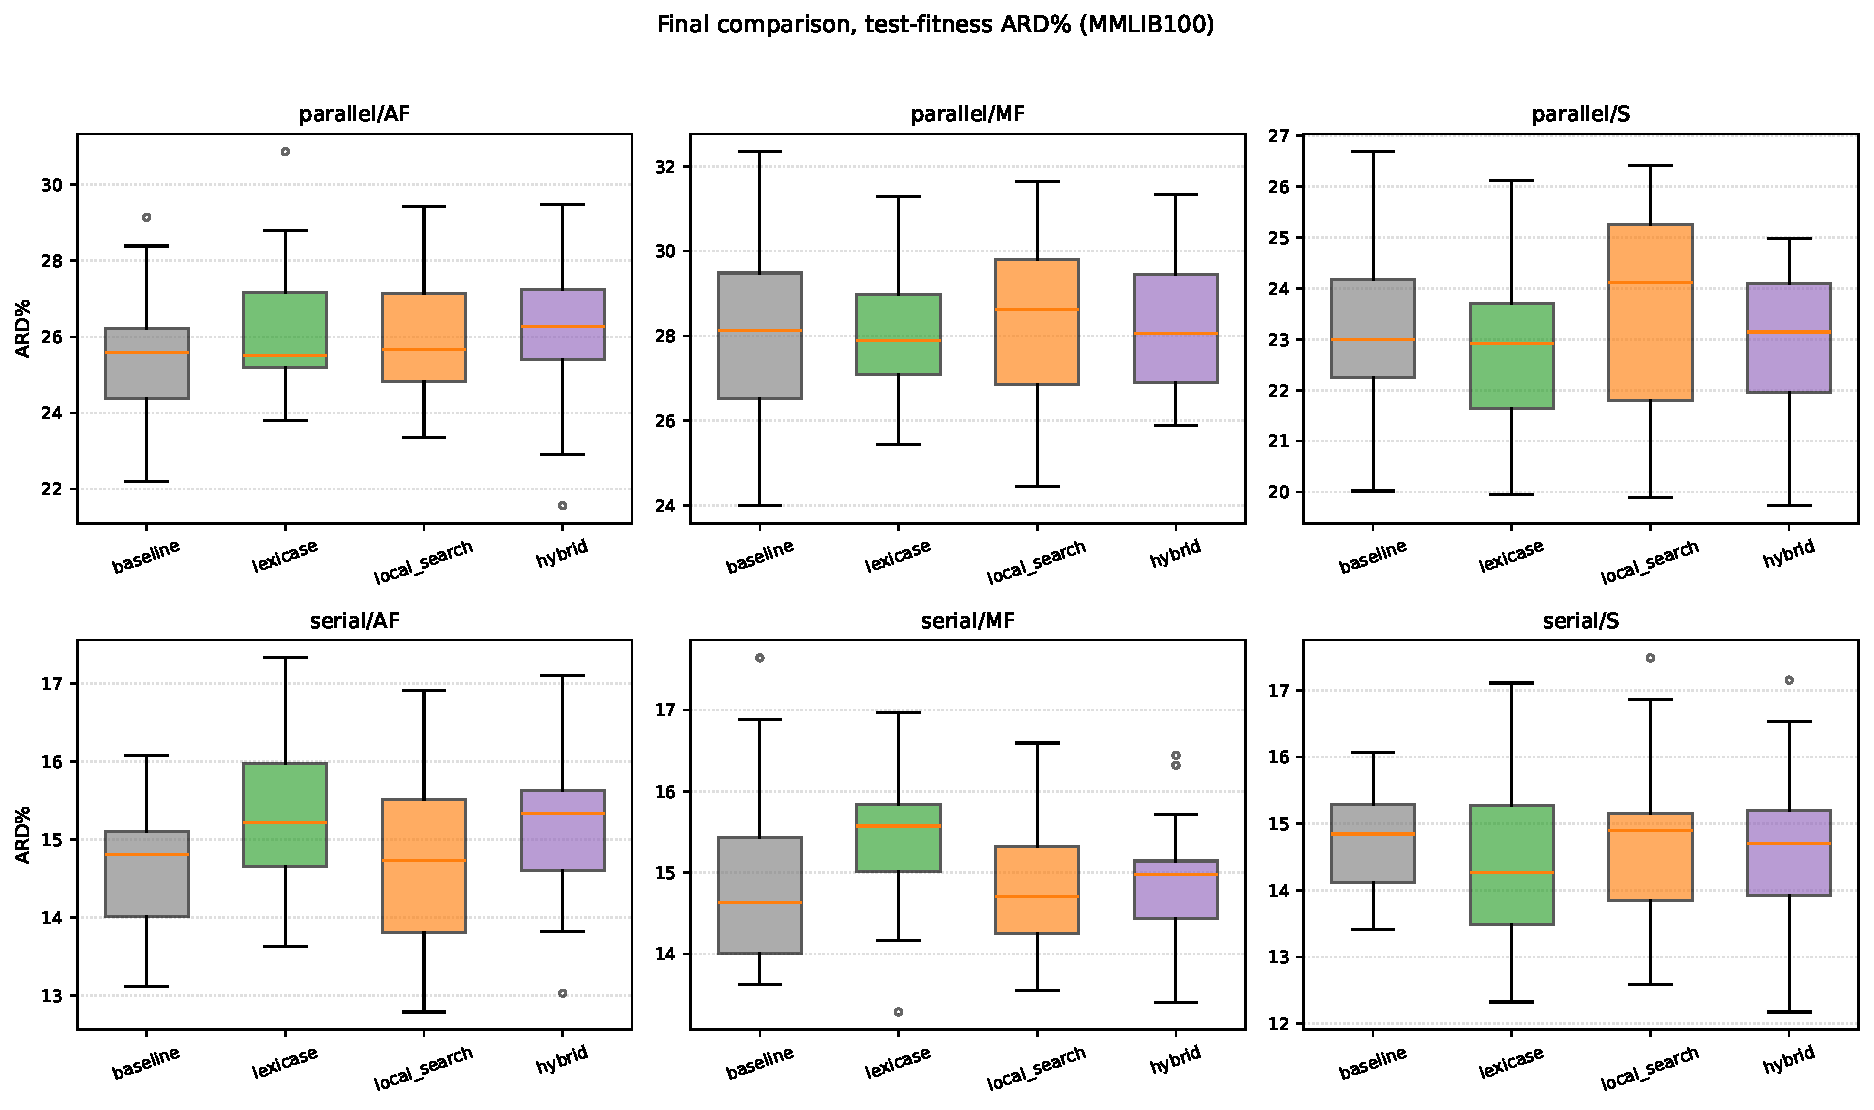
\includegraphics[width=0.95\textwidth]{img/generated/final_comparison_boxplot_mmlib100.pdf}
  \caption{Final comparison boxplot, all four jointly ranked conditions,
  MMLIB100, one panel per (SGS, strategy) cell, same layout as
  Figure~\ref{fig:final-comparison-boxplot}. Note local search's spread
  overlapping baseline's in every panel, consistent with
  Table~\ref{tab:method-rankings-mmlib100}'s non-significant Friedman test.}
  \label{fig:final-comparison-boxplot-mmlib100}
\end{figure}

A critical-difference diagram is deliberately \emph{not} presented for
MMLIB100's ranking, consistent with the convention fixed in
Section~\ref{subsec:statistical-methodology}: a CD diagram is only drawn
where the underlying Friedman test is itself significant, and neither
MMLIB100 Friedman test clears that bar (Table~\ref{tab:method-rankings-mmlib100}).

The joint ranking adds a finding that none of the three pairwise
subsections could show on its own: the Friedman test across the six cells
is significant ($p=0.0169$), so the difference between local search's
average rank (1.50) and hybrid's (3.83) is not attributable to chance, even
though neither individual pairwise comparison against baseline reached
significance in every cell. Two observations stand out. First, local
search alone achieves the best average test-fitness rank of the four, a
more favourable summary than Section~\ref{subsec:localsearch-eval}'s
cell-by-cell significance table might suggest on its own, precisely because
ranking rewards a method that is consistently a little better even where
no single cell clears the $p<0.05$ bar. Second, and more strikingly,
\emph{hybrid}, lexicase and local search combined, ranks worst of the four,
not best: Table~\ref{tab:lexicase-significance}-style pairwise tests (not
reproduced in full here for space) show hybrid significantly worse than
baseline on test fitness in three of six cells (all three under serial
SGS), against a single significant win under parallel/activity-first.
Combining the two individually defensible mechanisms does not add their
benefits; if anything, it compounds whatever is producing lexicase's
serial-SGS generalisation gap (Section~\ref{subsec:lexicase-eval}), since
hybrid inherits lexicase's selection mechanism on top of local search's own
refinement step. \changed{A plausible-looking combination of two components
that each showed some individual promise thus underperforms both
components individually, and is not recommended by this evidence as the
thesis's final proposed configuration.}

\textbf{Scalability validation.} This is the second, and more consequential,
instance in this chapter of an MMLIB50 finding not surviving the move to
MMLIB100. Table~\ref{tab:method-rankings-mmlib100} shows local search
falling from the \emph{best} average test-fitness rank on MMLIB50 (1.50) to
the \emph{worst} on MMLIB100 (2.83), with baseline itself now ranking best
(2.00); neither MMLIB100 Friedman test reaches significance, so, unlike
MMLIB50, the ranking differences at this scale are not distinguishable from
chance in the first place. Lexicase's relative position is more stable, it
ranks second-worst on MMLIB100 test fitness (2.50, tied with its own
MMLIB50 rank) while actually improving to the best rank on MMLIB100
\emph{training} fitness (1.67), consistent with
Section~\ref{subsec:lexicase-eval}'s finding that its training advantage is
real and, if anything, strengthens with scale even as its test advantage
does not. The practical implication is that this chapter's MMLIB50-only
final ranking, in particular its endorsement of local search as the
best-performing single condition, should not be read as a scale-independent
verdict: at MMLIB100, no condition in this four-way comparison
distinguishes itself from baseline with statistical confidence, and the
one candidate that appeared to (local search) \changed{owed its favourable
average rank to a consistent but individually non-significant advantage
across cells, an advantage that inverts once the same protocol is applied
to larger instances.}
Of the three comprehensive-stage candidates, this leaves NR terminals
(Section~\ref{subsec:nr-eval}), evaluated separately from this ranking for
the instance-set reasons already stated, as the only one whose evidence for
a real effect strengthens rather than weakens under scaling.

\textbf{Breakdown by instance characteristics.}
\changed{Because every test class corresponds to one OS/RF/RS combination
(Section~\ref{subsec:instance-sampling}), the per-class results show
directly how the conditions behave across instance characteristics.
Table~\ref{tab:per-class-breakdown} reports, for each of the ten MMLIB50
test instances, its indicators (computed directly from the instance; RS is
the mean over the two renewable resources) and the mean held-out deviation
of the four jointly ranked conditions (serial SGS, activity-first, 30
seeds, feasible runs). Two observations stand out. First, difficulty is
driven far more by the instance characteristics than by the choice of
condition: the tightly resource-constrained, high-RF classes
(\texttt{J5011}: OS 0.25, RF 1.00, RS 0.25; \texttt{J501};
\texttt{J5081}) dominate the aggregate ARD\%, while every condition
solves the loosely constrained classes ($\mathrm{RS} \ge 0.75$) at or
near the CPM bound. Second, the differences between conditions within a
class are small relative to the differences across classes, consistent
with the non-significant aggregate ranking at this scale; no condition is
systematically better on any particular OS/RF/RS regime.}

\begin{table}[htbp]
  \centering
  \small
  \shrinktofit{%
  \caption[Per-class breakdown of the final comparison]{\changed{Mean
  held-out deviation (\%) per test class, MMLIB50, serial SGS,
  activity-first, with each class's OS/RF/RS indicators computed from the
  instance. Rows are the ten stratified test instances (one per class).}}
  \label{tab:per-class-breakdown}
  \begin{tabular}{lrrrrrrr}
    \toprule
    \textbf{Instance} & \textbf{OS} & \textbf{RF} & \textbf{RS} & \textbf{Baseline} & \textbf{Lexicase} & \textbf{Local search} & \textbf{Hybrid} \\
    \midrule
    \texttt{J501\_5}  & 0.25 & 0.50 & 0.36 &  33.61 &  36.11 &  36.11 &  36.94 \\
    \texttt{J5011\_5} & 0.25 & 1.00 & 0.25 & 102.71 & 101.67 & 102.50 & 102.92 \\
    \texttt{J5021\_5} & 0.25 & 1.00 & 0.50 &   8.33 &   8.33 &   8.12 &   8.12 \\
    \texttt{J5031\_5} & 0.25 & 1.00 & 0.75 &   0.00 &   0.00 &   0.00 &   0.00 \\
    \texttt{J5041\_5} & 0.50 & 0.50 & 0.44 &   4.24 &   4.44 &   3.94 &   4.75 \\
    \texttt{J5051\_5} & 0.50 & 0.50 & 0.90 &   0.00 &   0.00 &   0.00 &   0.00 \\
    \texttt{J5061\_5} & 0.50 & 0.50 & 1.27 &   0.24 &   0.24 &   0.60 &   0.71 \\
    \texttt{J5071\_5} & 0.50 & 1.00 & 0.75 &   0.00 &   0.00 &   0.00 &   0.37 \\
    \texttt{J5081\_5} & 0.75 & 1.00 & 0.25 &  26.67 &  28.53 &  27.98 &  27.60 \\
    \texttt{J5091\_5} & 0.75 & 1.00 & 0.50 &   2.29 &   4.00 &   3.14 &   4.19 \\
    \bottomrule
  \end{tabular}%
  }
\end{table}

\subsection{Re-evaluation on the full 108-class test set}
\label{subsec:full108}

\changedB{Every test figure reported so far rests on a deliberately small
held-out set. To keep the comprehensive stage within the available compute
budget, each cell was trained and tested on a stratified subset of ten
classes out of each benchmark's 108 (Section~\ref{subsec:instance-sampling}),
and because that reduction applies to the test split as well, every mean test
ARD\% above is an average over just ten instances, one per sampled class. A
reasonable worry is that ten instances are too few to characterise a rule's
true test behaviour, and that some of the conclusions drawn above are
sensitive to which ten classes were sampled. This section addresses that
worry directly by re-evaluating the evolved rules on the complete 108-class
test set.}

\changedB{The procedure is cheap and changes nothing about how
the rules were produced. For every one of the 2160 cells (six conditions,
six SGS/strategy combinations, two benchmarks, thirty seeds) we take the
rule that cell already deployed, the validation-selected best individual that
produced its reported test figure, and re-evaluate it, with no further
evolution, on case 5 of every class from 1 to 108. This gives 108 held-out
test instances per benchmark in place of the original ten. The re-evaluation
reuses each condition's own conventions unchanged: the NR-preserving
instances and the NR terminal set for \texttt{nr} and \texttt{baseline\_nr},
the paper's renewable-only conversion for the other four conditions, and the
cell's own SGS and decision strategy. The metrics are unchanged as well:
ARD\%, the makespan's percentage deviation from the critical-path lower
bound averaged over the instances a rule schedules feasibly, and the
feasibility rate, the fraction of the 108 instances scheduled feasibly. No
population and no generations are involved, only one schedule construction
per instance, so the whole 2160-cell re-evaluation runs on a single
workstation without special resources.}

\begin{table}[htbp]
  \centering
  \small
  \caption[Full 108-class re-evaluation, renewable conditions]{\changedB{Test
  ARD\% on the full 108-class held-out set for the four conditions that share
  the renewable-only instance set. Baseline's ten-class figure is repeated
  from the tables above as the reference point for the shift; the other three
  conditions' ten-class figures lie within $1.2$ percentage points of
  baseline's in every cell and are omitted. All four conditions are
  $100\%$ feasible on both the ten-class and the 108-class test set.}}
  \label{tab:full108-renewable}
  \begin{tabular}{lrrrrr}
    \toprule
    & \multicolumn{2}{c}{\textbf{baseline}} & \textbf{lexicase}
    & \textbf{loc.\ search} & \textbf{hybrid} \\
    \cmidrule(lr){2-3}\cmidrule(lr){4-4}\cmidrule(lr){5-5}\cmidrule(lr){6-6}
    \textbf{SGS/strat.} & \textbf{10 cls} & \textbf{108 cls}
    & \textbf{108 cls} & \textbf{108 cls} & \textbf{108 cls} \\
    \midrule
    \multicolumn{6}{l}{\textit{MMLIB50}} \\
    Serial/AF   & 18.3 & 13.1 & 13.2 & 13.1 & 13.2 \\
    Serial/MF   & 18.1 & 13.1 & 13.0 & 13.1 & 13.1 \\
    Serial/S    & 18.3 & 13.1 & 13.3 & 13.3 & 13.5 \\
    Parallel/AF & 34.7 & 23.5 & 24.0 & 23.0 & 24.1 \\
    Parallel/MF & 36.0 & 24.7 & 24.8 & 24.9 & 24.7 \\
    Parallel/S  & 31.6 & 21.1 & 21.2 & 20.6 & 21.1 \\
    \midrule
    \multicolumn{6}{l}{\textit{MMLIB100}} \\
    Serial/AF   & 14.4 & 11.7 & 11.7 & 11.8 & 11.5 \\
    Serial/MF   & 14.6 & 11.9 & 11.8 & 11.9 & 11.6 \\
    Serial/S    & 14.6 & 11.8 & 11.9 & 11.9 & 11.9 \\
    Parallel/AF & 25.5 & 19.8 & 19.7 & 19.8 & 19.6 \\
    Parallel/MF & 28.0 & 21.3 & 21.1 & 21.3 & 21.1 \\
    Parallel/S  & 23.2 & 17.3 & 17.0 & 17.2 & 17.1 \\
    \bottomrule
  \end{tabular}
\end{table}

\changedB{Table~\ref{tab:full108-renewable} gives the outcome for the four
conditions on the renewable-only instances, and two facts hold across all
twelve cells. First, enlarging the test set from ten classes to 108 lowers
ARD\% everywhere, by $6.2$ percentage points on average and by between $2.1$
and $11.4$ points depending on the cell. \changedC{The shift is chiefly a
\changedD{sampling} effect: easy and hard instances are not represented in the ten
stratified classes in their true benchmark proportions, and the ten happen
to over-sample the tightly constrained, high-ARD\% end of the OS/RF/RS
grid (visible directly in Table~\ref{tab:per-class-breakdown}), whereas
the 108-class set contains every class and so restores the benchmark's
actual mix of easy and hard instances.} The ten-class test set was thus a
small and, as it turns out, somewhat pessimistic sample, so the absolute test
figures reported earlier are, if anything, conservative rather than
flattering. Second, and more important for the argument of this chapter, the
four conditions stay indistinguishable at full test scale exactly as they
were at ten classes: on 108 classes lexicase, local search, and hybrid each
remain within $0.65$ percentage points of baseline in every cell. The
near-null result for these three modifications on the renewable instances is
therefore not an artefact of the reduced test set; it survives evaluation on
the complete held-out distribution.}

\begin{table}[htbp]
  \centering
  \small
  \caption[Full 108-class re-evaluation, NR conditions]{\changedB{The NR pair
  on their NR-preserving instances. ARD\% is on the full 108-class test set;
  feasibility is shown for both the ten-class (\emph{feas.\ 10}) and the
  108-class (\emph{feas.\ 108}) sets so the change of scale is visible. Lower
  ARD\% and higher feasibility are better.}}
  \label{tab:full108-nr}
  \begin{tabular}{lrrrrrr}
    \toprule
    & \multicolumn{3}{c}{\textbf{\texttt{baseline\_nr}}}
    & \multicolumn{3}{c}{\textbf{NR terminals}} \\
    \cmidrule(lr){2-4}\cmidrule(lr){5-7}
    \textbf{SGS/strat.} & \textbf{ARD\%} & \textbf{feas.\,10}
    & \textbf{feas.\,108} & \textbf{ARD\%} & \textbf{feas.\,10}
    & \textbf{feas.\,108} \\
    \midrule
    \multicolumn{7}{l}{\textit{MMLIB50}} \\
    Serial/AF   & 126.4 & 70\% & 84\% & 88.4  & 84\% & 70\% \\
    Serial/MF   & 125.7 & 68\% & 84\% & 94.5  & 83\% & 75\% \\
    Serial/S    & 132.0 & 70\% & 89\% & 94.1  & 85\% & 85\% \\
    Parallel/AF & 115.8 & 67\% & 80\% & 107.2 & 85\% & 79\% \\
    Parallel/MF & 117.9 & 68\% & 83\% & 105.7 & 82\% & 79\% \\
    Parallel/S  & 120.0 & 67\% & 82\% & 113.6 & 83\% & 90\% \\
    \midrule
    \multicolumn{7}{l}{\textit{MMLIB100}} \\
    Serial/AF   & 116.1 & 85\% & 86\% & 87.6  & 98\% & 84\% \\
    Serial/MF   & 116.1 & 88\% & 88\% & 90.2  & 98\% & 87\% \\
    Serial/S    & 122.9 & 91\% & 89\% & 97.9  & 99\% & 96\% \\
    Parallel/AF & 111.1 & 78\% & 83\% & 93.8  & 89\% & 85\% \\
    Parallel/MF & 110.1 & 81\% & 85\% & 93.7  & 88\% & 82\% \\
    Parallel/S  & 118.7 & 81\% & 88\% & 97.8  & 87\% & 87\% \\
    \bottomrule
  \end{tabular}
\end{table}

\changedB{Table~\ref{tab:full108-nr} tells a more nuanced story for the NR
pair. The schedule-quality advantage of NR terminals is untouched by the
change of scale: their 108-class ARD\% is below \texttt{baseline\_nr}'s in
all twelve cells, by margins from about $6$ to nearly $40$ percentage points,
in line with the ten-class result of Section~\ref{subsec:nr-eval}. What does
not carry over cleanly is the feasibility advantage. On the ten-class test
set NR terminals scheduled a larger fraction of instances feasibly than
\texttt{baseline\_nr} in every one of the twelve cells; on the full 108-class
set this gap closes to near-parity on MMLIB100 and reverses on MMLIB50, where
NR terminals' feasibility sits at or below \texttt{baseline\_nr}'s in five of
the six cells. The reading consistent with both metrics is that NR terminals
produce markedly better schedules on the instances they solve, but that part
of their feasibility gain on the ten sampled classes is an in-distribution
effect: the rule, evolved on three cases of those same ten classes, extends
its quality advantage to the 98 unseen classes far more reliably than it
extends its feasibility advantage. This qualifies, without overturning, the
feasibility claim of Section~\ref{subsec:nr-eval}; the central and larger
schedule-quality result is unaffected.}

\changedB{The feasibility reversal appears only at the larger test scale
because the ten sampled classes are the very classes each rule was trained
on, so the ten-class figure measures in-distribution feasibility, while the
98 classes added to reach 108 are unseen. Splitting the 108-class feasibility
into these two parts (Table~\ref{tab:full108-nr-generalisation}) isolates the
effect. On the ten seen classes NR terminals are far more feasible than
\texttt{baseline\_nr} ($84\%$ against $68\%$ on MMLIB50, $93\%$ against
$84\%$ on MMLIB100), which is the gain reported in
Section~\ref{subsec:nr-eval}. On the 98 unseen classes that gain disappears:
NR terminals fall to $79\%$ and $86\%$ while \texttt{baseline\_nr} rises to
$85\%$ and $87\%$, so the two are level or NR terminals sit marginally
behind. The asymmetry is mechanistic. \texttt{baseline\_nr} cannot see the
non-renewable state, so it has no class-specific budget management to overfit
and its feasibility simply tracks class difficulty, and because the sampled
ten classes are harder than the benchmark average (the same reason ARD\%
falls when the test set is enlarged) its feasibility rises on the broader
set. NR terminals give the rule exactly the expressiveness needed to secure
feasibility on the classes it trains on, and that part of the benefit does
not carry to unseen classes. Schedule quality transfers because a good
relative priority ordering generalises across classes; the absolute
non-renewable budget thresholds that decide feasibility do not.}

\begin{table}[htbp]
  \centering
  \small
  \caption[Feasibility on seen versus unseen classes]{\changedB{Feasibility
  rate of the NR pair split into the ten training-adjacent (seen) classes and
  the 98 unseen classes that make up the rest of the 108-class test set.
  The \emph{all 108} column is the feasibility of
  Table~\ref{tab:full108-nr}. NR terminals' feasibility advantage is confined
  to the seen classes.}}
  \label{tab:full108-nr-generalisation}
  \begin{tabular}{llrrr}
    \toprule
    \textbf{Benchmark} & \textbf{Condition} & \textbf{seen (10)}
    & \textbf{unseen (98)} & \textbf{all 108} \\
    \midrule
    \multirow{2}{*}{MMLIB50}
      & \texttt{baseline\_nr} & 68\% & 85\% & 84\% \\
      & NR terminals          & 84\% & 79\% & 80\% \\
    \addlinespace
    \multirow{2}{*}{MMLIB100}
      & \texttt{baseline\_nr} & 84\% & 87\% & 86\% \\
      & NR terminals          & 93\% & 86\% & 87\% \\
    \bottomrule
  \end{tabular}
\end{table}

\changedC{\textbf{Breakdown by instance characteristics.} With 108 test
instances per benchmark, the re-evaluation is also large enough to be
split by instance characteristics, which the ten-class test set was not.
Because every class realises one OS/RF/RS combination and the indicators
are computed directly from each instance (as in
Table~\ref{tab:per-class-breakdown}),
Tables~\ref{tab:full108-os}--\ref{tab:full108-rs} report the same
108-class test results separately for every value of each indicator: each
entry is the mean test ARD\% computed only over the instances with the
given OS, RF, or RS value, pooled across all six (SGS, strategy) cells
and 30 seeds. OS and RF take exactly three and two values on the MMLIB
grid; RS is continuous, so it is grouped into tight
($\mathrm{RS} \le 0.5$), medium ($0.5 < \mathrm{RS} \le 1$) and
effectively unconstrained ($\mathrm{RS} > 1$) instances. The four
renewable-instance conditions are $100\%$ feasible everywhere, so only
ARD\% is shown for them; for the NR pair, which runs on the NR-preserving
instances and is not comparable in magnitude to the other four, the
feasibility rate over the group is given in parentheses.}

\begin{table}[htbp]
  \centering
  \small
  \caption[108-class breakdown by order strength]{\changedC{Test ARD\%
  on the full 108-class set, computed only over instances with the given
  order strength (OS), pooled over all six (SGS, strategy) cells and 30
  seeds. NR-pair entries (their own NR-preserving instance set) carry the
  group's feasibility rate in parentheses; the four renewable conditions
  are $100\%$ feasible throughout.}}
  \label{tab:full108-os}
  \begin{tabular}{lrrr}
    \toprule
    \textbf{Condition} & $\mathrm{OS} = 0.25$ & $\mathrm{OS} = 0.50$ & $\mathrm{OS} = 0.75$ \\
    \midrule
    \multicolumn{4}{l}{\textit{MMLIB50}} \\
    Baseline & 23.6 & 18.3 & 12.3 \\
    Lexicase & 23.8 & 18.4 & 12.6 \\
    Local search & 23.6 & 18.2 & 12.2 \\
    Hybrid & 24.0 & 18.3 & 12.5 \\
    \texttt{baseline\_nr} & 122.0 (85\%) & 125.5 (84\%) & 126.6 (82\%) \\
    NR terminals & 106.9 (83\%) & 103.0 (81\%) & 97.5 (75\%) \\
    \midrule
    \multicolumn{4}{l}{\textit{MMLIB100}} \\
    Baseline & 14.8 & 19.1 & 13.0 \\
    Lexicase & 14.5 & 18.8 & 13.2 \\
    Local search & 14.8 & 19.1 & 13.1 \\
    Hybrid & 14.5 & 18.9 & 13.0 \\
    \texttt{baseline\_nr} & 115.0 (88\%) & 126.9 (88\%) & 109.4 (83\%) \\
    NR terminals & 95.9 (95\%) & 99.9 (87\%) & 86.1 (79\%) \\
    \bottomrule
  \end{tabular}
\end{table}

\begin{table}[htbp]
  \centering
  \small
  \caption[108-class breakdown by resource factor]{\changedC{Test ARD\%
  on the full 108-class set, computed only over instances with the given
  resource factor (RF); layout as in Table~\ref{tab:full108-os}.}}
  \label{tab:full108-rf}
  \begin{tabular}{lrr}
    \toprule
    \textbf{Condition} & $\mathrm{RF} = 0.50$ & $\mathrm{RF} = 1.00$ \\
    \midrule
    \multicolumn{3}{l}{\textit{MMLIB50}} \\
    Baseline & 8.2 & 28.0 \\
    Lexicase & 8.3 & 28.2 \\
    Local search & 8.2 & 27.8 \\
    Hybrid & 8.3 & 28.3 \\
    \texttt{baseline\_nr} & 104.8 (83\%) & 144.0 (85\%) \\
    NR terminals & 83.9 (77\%) & 120.0 (83\%) \\
    \midrule
    \multicolumn{3}{l}{\textit{MMLIB100}} \\
    Baseline & 6.1 & 25.1 \\
    Lexicase & 6.0 & 25.0 \\
    Local search & 6.2 & 25.1 \\
    Hybrid & 5.9 & 25.1 \\
    \texttt{baseline\_nr} & 95.4 (83\%) & 137.4 (90\%) \\
    NR terminals & 76.7 (85\%) & 110.9 (89\%) \\
    \bottomrule
  \end{tabular}
\end{table}

\begin{table}[htbp]
  \centering
  \small
  \caption[108-class breakdown by resource strength]{\changedC{Test ARD\%
  on the full 108-class set, computed only over instances in the given
  resource-strength (RS) range; layout as in
  Table~\ref{tab:full108-os}.}}
  \label{tab:full108-rs}
  \begin{tabular}{lrrr}
    \toprule
    \textbf{Condition} & $\mathrm{RS} \le 0.5$ & $0.5 < \mathrm{RS} \le 1$ & $\mathrm{RS} > 1$ \\
    \midrule
    \multicolumn{4}{l}{\textit{MMLIB50}} \\
    Baseline & 43.7 & 4.6 & 0.5 \\
    Lexicase & 43.9 & 4.8 & 0.4 \\
    Local search & 43.6 & 4.5 & 0.4 \\
    Hybrid & 44.1 & 4.7 & 0.4 \\
    \texttt{baseline\_nr} & 157.9 (78\%) & 109.5 (87\%) & 103.0 (90\%) \\
    NR terminals & 135.0 (75\%) & 87.8 (81\%) & 80.2 (86\%) \\
    \midrule
    \multicolumn{4}{l}{\textit{MMLIB100}} \\
    Baseline & 31.2 & 2.8 & 0.5 \\
    Lexicase & 30.9 & 2.9 & 0.5 \\
    Local search & 31.3 & 2.8 & 0.5 \\
    Hybrid & 31.1 & 2.7 & 0.3 \\
    \texttt{baseline\_nr} & 140.5 (83\%) & 99.3 (90\%) & 97.1 (87\%) \\
    NR terminals & 113.8 (81\%) & 80.4 (91\%) & 77.2 (96\%) \\
    \bottomrule
  \end{tabular}
\end{table}

\changedC{Three observations follow. First, difficulty is driven
overwhelmingly by the resource indicators, not by the network shape:
moving from $\mathrm{RF} = 0.50$ to $\mathrm{RF} = 1.00$ roughly triples
the renewable conditions' ARD\% (8.2 to 28.0 on MMLIB50), and moving
from tight to effectively unconstrained RS spans almost the entire
observed range (43.7 down to 0.5), while OS produces the smallest and
least systematic differences (on MMLIB100 the middle level
$\mathrm{OS} = 0.50$ is the hardest). Second, the four renewable
conditions remain indistinguishable \emph{within every single indicator
level}: the largest spread between them in any cell of the three tables
is $0.5$ percentage points, so the earlier per-class observation that no
condition is systematically better on any particular OS/RF/RS regime
(Table~\ref{tab:per-class-breakdown}) holds on the complete test
distribution, not just the ten stratified classes. Third, NR terminals'
schedule-quality advantage over \texttt{baseline\_nr} is present at
every value of every indicator on both benchmarks (by 15--29 points on
MMLIB50 and 19--27 points on MMLIB100), while their MMLIB50 feasibility
shortfall is spread fairly evenly across the levels rather than
concentrated in one regime, consistent with
Table~\ref{tab:full108-nr-generalisation}'s reading that the shortfall
follows class identity (seen versus unseen), not any particular
instance characteristic.}

\changedD{The feasibility rates of Table~\ref{tab:full108-rs} show one
further pattern: as RS grows and the renewable constraints loosen, the
NR-aware rules schedule an increasing share of instances feasibly, on
MMLIB100 rising from $81\%$ on the tight instances to $96\%$ on the
effectively unconstrained ones, while \texttt{baseline\_nr} shows no such
progression there ($83$--$90\%$, with no gain at $\mathrm{RS} > 1$). This
is what the terminals' mechanism predicts: the looser the renewable
constraints, the more feasibility is decided by the non-renewable budget
alone, which is precisely the state the NR terminals expose and the
baseline cannot see. On MMLIB50 both conditions' feasibility improves with
RS at a similar rate, so the separation is clearly visible only at the
larger instance size.}

Taken together, Sections~\ref{sec:parameter-sensitivity}
through~\ref{sec:benchmark-comparison} tell a coherent
story. Of a wide field of candidate ideas, screened
cheaply and then narrowed to three, only NR terminals produced a result
that is large, consistent, and free of the SGS-dependent reversals that
qualify the other two; lexicase selection and critical-path local search
each show a genuine, mechanistically interpretable signal, but a signal
that is smaller, direction-dependent, and, in lexicase's case, prone to not
generalising past the training set; and the naive combination of the two
weaker methods performs worse than either alone. Chapter~\ref{chap:conclusion}
takes up the question of what this pattern of results implies for the
thesis's research questions and for GPHH-based scheduling research more
broadly.

\section{Complexity analysis and limitations}
\label{sec:complexity-limitations}

The cost of a single GP run is dominated by fitness evaluation: each of the
$N_{\text{pop}}$ individuals must decode a schedule via the SGS on every
training instance, once per generation, so a single run's cost scales as
$O(N_{\text{pop}} \times N_{\text{gen}} \times N_{\text{inst}} \times
C_{\text{decode}})$, where $C_{\text{decode}}$ itself grows with the
number of activities and modes per instance. This is why MMLIB100 costs
substantially more per run
than MMLIB50 at the same population and generation budget, purely from
doubling the activity count, and why \changed{the training times reported
by Tian et al.~\cite{Tian2024GPHH}} range from a few
hundred seconds for parallel SGS on MMLIB50 up to tens of thousands of
seconds for serial SGS on the largest MMLIB+ instances at the full
pop=1\,000/gen=50 budget. \changed{This cost structure is why the
comprehensive stage evaluates every condition on a
stratified $n_{\text{classes}}=10$ subsample of each dataset's full 108
classes rather than on all of them
(Section~\ref{subsec:instance-sampling}): all planned runs on that
subsample were completed, but reproducing the paper's
own full-class evaluation for the baseline alone, let alone six conditions
across two SGS types and three decision strategies, \changedC{would have
taken several hundred days of computation, more than could be completed
within the time frame of this thesis (MetaCentrum itself imposes no such
limit; the constraint was the thesis's schedule)}.}

\changed{The realised cost of the comprehensive stage can be stated
exactly, since every result file records its own wall-clock running time.
The 2\,160 comprehensive-stage runs (1\,080 per benchmark) took a combined
$17\,187$ hours of wall-clock time, about $716$ days, corresponding to
roughly $5\,700$ CPU-days at the 8 cores allocated per run. A single
MMLIB50 run took $3.4$ hours on average (median $2.3$, range
$0.7$--$25.1$); a single MMLIB100 run took $12.5$ hours on average (median
$10.2$, range $2.8$--$55.9$), confirming the cost increase from doubling
the instance size. By condition, \texttt{local\_search} and \texttt{hybrid}
were indeed the most expensive, averaging $4.5$--$4.6$ hours per MMLIB50
run and $15.7$--$16.3$ hours per MMLIB100 run against the baseline's
$2.8$ and $10.0$ hours; by decoding scheme, serial-SGS runs took roughly
twice as long as parallel ones on average ($5.0$ versus $1.8$ hours on
MMLIB50, $16.7$ versus $8.4$ hours on MMLIB100). Including the
exploratory stage, preliminary and repeated jobs, and all side
experiments, the MetaCentrum account used for this thesis executed
$30\,287$ jobs consuming roughly $11\,600$ CPU-days in total. These times
were measured on heterogeneous, scheduler-assigned grid nodes
(Table~\ref{tab:hw-sw-config}) and are therefore indicative rather than
exactly comparable across runs.}

The three proposed extensions add comparatively little to this base cost,
but not equally so. NR terminals are the cheapest: each of the three added
terminals is a constant-time lookup against a per-instance cache computed
once before the run begins, so the per-individual evaluation cost is
essentially unchanged from the baseline. Epsilon-lexicase selection is
more expensive per selection event than tournament selection, since it may
filter over as many training cases as it takes to narrow the candidate
pool to one survivor, rather than comparing a fixed, small tournament
sample, though this cost is still minor relative to fitness evaluation
itself. Critical-path local search is the most expensive of the three: its
hill-climb runs for up to ten iterations on the top 8\% of the population,
every generation, and each iteration re-decodes the candidate schedule to
check feasibility, which \changed{made \texttt{local\_search} and
\texttt{hybrid} the most expensive conditions in the walltime estimates
used for PBS job scheduling. One combination of the full
paper-scale grid, the \texttt{hybrid} condition under serial SGS with the
mode-first strategy on the largest MMLIB+ instances, was excluded from the
matrix entirely on this basis: \changedC{even a single seed's estimated
running time was so long that the full 30-seed cell could not have
finished before this thesis was due}.}

Two further limitations accompany the cost
model. First, every comprehensive-stage run in this chapter used
population 1\,000 and 50 generations, matching the paper's own
configuration; whether the qualitative pattern of results, in particular
lexicase's SGS-dependent train/test gap and local search's parallel/serial
asymmetry, holds at a substantially different population or generation
budget is not established here. Second, the cost model above is
specific to this thesis's own MetaCentrum allocation
(Table~\ref{tab:hw-sw-config}) and
should not be read as a general claim about how these extensions would
scale on different hardware or under a different parallelisation strategy
than the 8-core, population-level parallelism used throughout\changed{;
moreover, individual jobs were placed by the scheduler on heterogeneous
grid nodes, so even the running times observed within this thesis are only
approximately comparable to one another.}
